% Shared preamble for the MIRAGE report and supplementary document
\documentclass[10pt,a4paper,twocolumn]{article}
\usepackage[a4paper,top=1.6cm,bottom=1.6cm,left=1.5cm,right=1.5cm,columnsep=0.7cm]{geometry}
\usepackage[T1]{fontenc}
\usepackage[utf8]{inputenc}
\usepackage{times}
\usepackage{microtype}
\usepackage{graphicx}
\usepackage{booktabs}
\usepackage{array}
\usepackage{tabularx}
\usepackage{longtable}
\usepackage{caption}
\usepackage{subcaption}
\usepackage{amsmath}
\usepackage{siunitx}
\usepackage{xcolor}
\usepackage{enumitem}
\usepackage{titlesec}
\usepackage{hyperref}
\usepackage{xurl}
\usepackage{float}
\usepackage{setspace}

\definecolor{mirageblue}{HTML}{1F4E79}
\definecolor{mirageink}{HTML}{222222}
\hypersetup{colorlinks=true,linkcolor=mirageblue,citecolor=mirageblue,urlcolor=mirageblue,pdftitle={MIRAGE: Measuring the Impact and Reality of Rainwater Harvesting Mandates}}

\titleformat{\section}{\normalfont\fontsize{10.5}{12}\bfseries\color{mirageblue}}{\thesection}{0.5em}{}
\titleformat{\subsection}{\normalfont\fontsize{10}{12}\bfseries}{\thesubsection}{0.5em}{}
\titlespacing*{\section}{0pt}{6pt plus 2pt minus 1pt}{3pt}
\titlespacing*{\subsection}{0pt}{4pt plus 1pt minus 1pt}{2pt}
\captionsetup{font=small,labelfont=bf,skip=3pt}
\setlist{nosep,leftmargin=1.2em}
\setlength{\parskip}{2pt}
\setlength{\parindent}{0pt}
\sisetup{group-separator={,},group-minimum-digits=4}
\renewcommand{\arraystretch}{1.12}
\newcommand{\inr}{Rs}

\usepackage{needspace}
\usepackage{listings}
\lstset{basicstyle=\ttfamily\fontsize{6.6pt}{7.6pt}\selectfont,breaklines=true,breakatwhitespace=false,numbers=left,numberstyle=\tiny\color{gray},numbersep=5pt,frame=single,framerule=0.3pt,rulecolor=\color{gray!60},showstringspaces=false,keywordstyle=\color{mirageblue},commentstyle=\color{gray!80!black}\itshape,stringstyle=\color{violet!70!black},columns=fullflexible,keepspaces=true,postbreak=\mbox{\textcolor{gray}{$\hookrightarrow$}\space},literate={₹}{{Rs}}1 {×}{{x}}1 {→}{{->}}1 {−}{{-}}1 {ρ}{{rho}}1 {²}{{2}}1 {³}{{3}}1 {≥}{{>=}}1 {≤}{{<=}}1 {≈}{{~}}1 {–}{{-}}1 {—}{{-}}1 {“}{{"}}1 {”}{{"}}1 {‘}{{'}}1 {’}{{'}}1 {é}{{e}}1 {…}{{...}}1}
\geometry{top=2cm,bottom=2cm,left=1.8cm,right=1.8cm}
\begin{document}
\onecolumn
\begin{center}
{\LARGE\bfseries\color{mirageblue} MIRAGE: Supplementary Information, with code}\\[4pt]
{\large Measuring the Impact and Reality of Rainwater Harvesting Mandates. A meta-analysis of rooftop rainwater harvesting performance in Indian cities}\\[6pt]
Vedant Abhangrao (23B2262) \,|\, Nilay Shahapure (23B2206) \,|\, Arjun Jhunjhunwala (23B1245) \,|\, Yash Krishnani (23B1240)\\[2pt]
{\small CM617 Sustainability Principles and Practices, IIT Bombay. October 2026.}
\end{center}

\tableofcontents

\section{Data and code supplied with this report}
\textbf{Code repository.} All data, code, figures and the LaTeX sources of this report are also available at \url{https://github.com/nilay-shahapure/MIRAGE_CM617}. The repository contains the same files as the submission folder, with a script that rebuilds every number, figure and PDF from the source extraction tables.

The submission folder contains, besides this document and the main report: the harmonised dataset (performance observations with computed potential and ratios, cost rows with deflation and levelised cost, functionality estimates, installation figures, failure-mode counts, the mandate table, the screening log and the price-index series used for deflation); the source extraction tables, one row per source record, each carrying the URL and the sentence or field values taken from the page for every number used, together with verbatim extracts from the two CGWB documents and a codebook for every column; the Python scripts that rebuild the dataset, the statistics, the figures and the tables in this document from the source extraction tables (run in the order dataset, analysis, tables); and a results summary listing every number quoted in the report.

\section{Screening and inclusion}
The work was organised as four parallel searches, called strands below: performance (yield against potential), cost, functionality and failure modes, and mandates. The flow diagram and the log give the counts for each.
\begin{figure}[H]\centering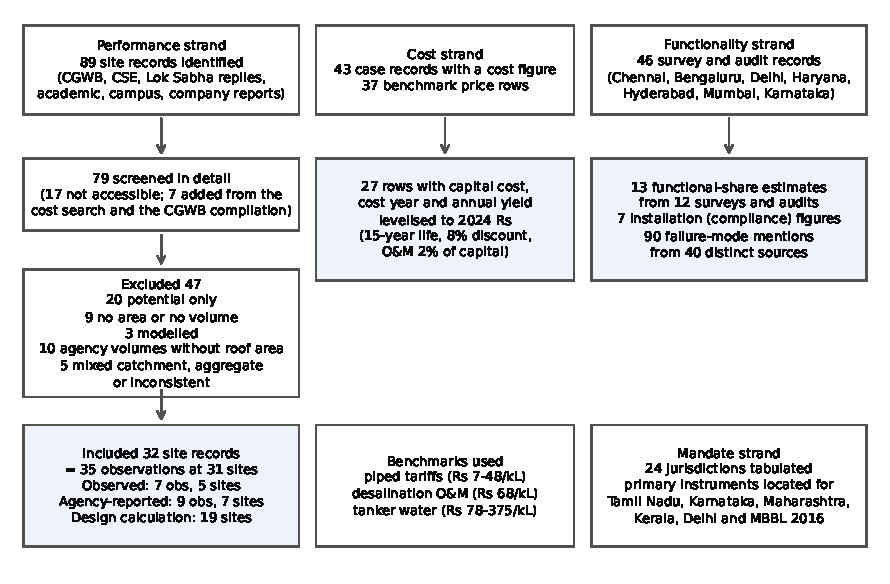
\includegraphics[width=0.95\textwidth]{../figures/figS4_screening_flow.pdf}
\caption{Screening and inclusion flow for the four research strands.}\end{figure}
{\scriptsize\setlength{\tabcolsep}{3pt}
\begin{longtable}{p{13cm} r}
\caption{Screening and inclusion log (counts behind the flow diagram above).}\label{tab:screen}\\
\toprule
\textbf{Step} & \textbf{Count}\\ \midrule\endfirsthead
\toprule \textbf{Step} & \textbf{Count}\\ \midrule\endhead
\bottomrule\endfoot
Performance strand: site records identified (CGWB, CSE, Lok Sabha replies, academic, campus and company reports) & 89\\
Performance strand: records not accessible (documents that could not be opened or were paywalled) & 17\\
Performance strand: records screened in detail (72 from the performance search, 6 CSE model projects from the cost search, 1 case read directly from the CGWB 2011 compilation) & 79\\
Excluded: potential only (no actual volume reported) & 20\\
Excluded: no catchment area or no volume & 9\\
Excluded: modelled volumes (JNTU Hyderabad, 3 structures) & 3\\
Excluded: agency volumes with no roof area (Lok Sabha 2004 list) & 10\\
Excluded: mixed or non-roof catchment, aggregate, or internally inconsistent & 5\\
Included site records & 32\\
Included observations (some sites have several years) & 35\\
Included as observed volumes (instrument or tank record named) & 7\\
Included as agency-reported volumes & 9\\
Included as design calculations (CSE model projects and CGWB design note) & 19\\
Cost strand: case records screened & 43\\
Cost strand: rows with both capital cost and annual yield and a cost year, used for levelised cost & 27\\
Cost strand: benchmark price rows & 37\\
Functionality strand: survey records screened & 46\\
Functionality strand: surveys with a measured functional / defunct split & 13\\
Functionality strand: city compliance (installation) figures & 7\\
Failure-mode mentions extracted & 90\\
Failure-mode distinct sources & 40\\
Failure-mode categories after collapsing & 11\\
Mandate jurisdictions tabulated & 24\\
\end{longtable}}


\paragraph{Inclusion rules for the performance strand.} A record entered the ratio analysis if it reported (i) a roof or whole-site catchment area, (ii) an actual harvested, collected or recharged volume for a stated period, and (iii) rainfall for the site or a city for which an IMD normal exists. Records reporting only design potential, only a storage capacity, only a structure count, or volumes for aggregated multi-site portfolios were excluded. Rows were graded by one mechanical rule into three evidence tiers: observed, if the source names a flow meter, a measuring device at the recharge well or a tank-filling record for that site; agency-reported, if an agency states an annual volume with no instrument named, or states it as a share of estimated runoff; design-calculated, if the source itself labels the figure a design calculation. The rule puts both CGWB Maharashtra demonstrations (Ramtek and Warud) in the observed tier, because CGWB describes an identical pipe train with a flow meter for both and uses the same sentence (``As per estimation, a total of X cu. m of rain was received on the roof of the building, out of which Y cu. m was actually recharged'') for both. Warud's Y is a round 90\% of X, which may be an assumed share; the main report therefore gives the result both ways (Table~\ref{tab:stats}). Shram Shakti Bhawan, whose CGWB figure is labelled ``expected recharge'', is design-calculated. The JNTU Hyderabad rows (modelled monthly volumes equal to rainfall $\times$ area $\times$ 0.9) were excluded as modelled rather than reported.

\paragraph{Harmonisation choices.} Theoretical potential $P = A \times R \times C/1000$ with $C = 0.80$. The CGWB (2007) manual gives 0.7 for concrete, 0.75 tiled, 0.8 asbestos and 0.9 GI sheet (Table 7.2, verified in the manual); the CGWB/National Water Mission 2020 guide gives 0.75 to 0.95 for roofs. Most included roofs are RCC; 0.80 is the midpoint of the manual's range and the value used in the CGWB 2003 rooftop tables and the midway check-in. The 0.70 and 0.90 columns in Table~\ref{tab:perf} and the sensitivity figure below show that the tier medians move by a few points but the ordering does not change. Rainfall: site-year where reported (Goa 2010, Bhubaneswar 2004 to 2006); rain received on the roof divided by area where the source reports it that way (Ramtek, Warud); the source's own city average where that is what the source used (CSE pages); IMD 1991-2020 normals otherwise. No IMD normal was located for Chandigarh, so the CSE figure (1,059.3 mm) is used for both Chandigarh cases; using the CGWB district normal (742 mm) instead raises both ratios further above 100\%, which does not change the conclusion that they are design-derived. For Ramtek the implied rainfall (215.7 m$^3$ over 360 m$^2$ = 599 mm) is well below the taluka average of 1,043.7 mm, so the monitored period was probably not a full year; using the taluka average would lower the Ramtek ratio from 11\% to 6\%. Catchment: for the CSE model projects the only area given is ``total rooftop and surface area'', so the design-calculated potentials apply a roof coefficient to roof plus paved and open ground; this is why that tier is used only as the design-share reference and not in the observed versus agency-reported comparison.

\section{Reconciliation with the midway check-in}
The midway check-in is the mid-term progress report submitted earlier in the course. The table below compares each of its six cases with the final dataset.
{\scriptsize\setlength{\tabcolsep}{3pt}
\begin{longtable}{p{2.3cm} p{3.4cm} p{4.6cm} p{5.6cm}}
\caption{Reconciliation of the six midway check-in cases with the final dataset. All six are retained; ratios were recomputed with one stated runoff coefficient and a stated rainfall basis.}\label{tab:recon}\\
\toprule
\textbf{Case} & \textbf{Midway check-in} & \textbf{Final} & \textbf{Reason for change}\\ \midrule\endfirsthead
\toprule \textbf{Case} & \textbf{Midway check-in} & \textbf{Final} & \textbf{Reason for change}\\ \midrule\endhead
\bottomrule\endfoot
KITS Ramtek & about 9\% (19 of 215.7 m$^3$ received) & 11\% (19 kL against potential 172.6 kL at C = 0.80); 8.8\% of rain received; observed tier & Numbers verified word for word in CGWB (2011) p.73; the midway ratio divided by gross rain, the final divides by potential (rain $\times$ 0.8). The implied rainfall (599 mm) is below the Ramtek taluka average of 1,043.7 mm, so the monitored period was probably not a full year; with the taluka average the ratio would be 6\%.\\
Goa University & 61--76\% (900 kL, about 400 m$^2$) & 76\% in 2010 (3.7 m rainfall); 28\% in 2008 (partial year) and 19\% in 2009 using the IMD Panaji normal & Midway used a range of runoff coefficients; final fixes C = 0.80 and adds the two earlier years reported in the same CSE table.\\
BEL Bengaluru & 63--75\% (about 1,100 kL recharged) & 64\% (1,100 kL, 2,000 m$^2$, IMD Bengaluru normal 1,077.6 mm) & Source says the water is harvested and stored for DM-water production, so the system type is storage, not recharge as the midway said.\\
Panjab University & about 79\% (1,985 m$^3$) & 112\% (2,100 m$^2$, 1,059.3 mm, C = 0.80); agency-reported tier & The midway figure used an unstated area or rainfall. The Lok Sabha source gives the volume as ``93\% of total generated runoff'', i.e. a design share, which is why the ratio exceeds 100\%.\\
Warud & 90\% (derived from runoff assumption) & 112\% against potential; 90\% of rain received; observed tier by the stated rule (flow meter named), with a sensitivity case grading it agency-reported & Confirmed in CGWB (2011) p.73 (500 m$^2$, 311.30 m$^3$ received, 280.17 m$^3$ recharged). The CGWB wording is identical to Ramtek, so one rule must grade both the same way; the round 90\% suggests an assumed share, which is why both gradings are reported.\\
IIT Delhi Block VI & not comparable (rainfall NR) & 82\% using the IMD Safdarjung normal (762.3 mm); agency-reported tier, rainfall basis flagged & Confirmed in CGWB (2011) p.44 (830 m$^3$ from 1,660 m$^2$). Rainfall period still not reported, so the ratio is indicative.\\
Umaid Heritage, Sri Aurobindo Ashram, PAU Ludhiana & supplementary (mixed catchments or calculated) & Umaid Heritage excluded (110-acre mixed catchment, internal inconsistency 21.1 vs 2.1 ML); Sri Aurobindo Ashram included as a design calculation (43\% of potential); PAU excluded (no roof area) & As the midway said: these are not comparable rooftop cases.\\
\end{longtable}}

The midway text also said that ``around ten studies reported only estimated or design-stage potential''; the final screening found 20 such records. It said ``over 50 sources'' were screened; the final count is 79 performance records plus 43 cost and 46 functionality records. Two items from the Milestone 1 plan were not carried through: system age as a regression predictor (year of installation is recorded where known, but too few observations have a stated study year to compute age), and campus sustainability reports as a data source (the Infosys and Wipro reports give portfolio totals without catchment areas and were excluded).

\needspace{6\baselineskip}\section{Performance dataset}
{\scriptsize\setlength{\tabcolsep}{3pt}
\begin{longtable}{l p{2.7cm} l >{\raggedright\arraybackslash}p{1.6cm} r p{1.6cm} p{1.1cm} r r r l}
\caption{Performance dataset: all 35 observations. Evidence: Observed (instrument or tank record named), Agency (agency-reported, no instrument named), Design (design calculation). Potential uses runoff coefficient 0.80; the last column gives the ratio for C = 0.70 and 0.90. Rainfall basis: site-year (reported for that site and year), site-avg (average quoted by the source), city-avg (CSE city figure), city-normal (IMD normal), implied (rain received on roof divided by area).}\label{tab:perf}\\
\toprule
\textbf{No.} & \textbf{Site} & \textbf{Evidence} & \textbf{Type / system} & \textbf{Area m$^2$} & \textbf{Rain mm (basis)} & \textbf{Year} & \textbf{Vol. kL} & \textbf{Pot. kL} & \textbf{Ratio \%} & \textbf{C 0.7--0.9}\\ \midrule\endfirsthead
\toprule \textbf{No.} & \textbf{Site} & \textbf{Evidence} & \textbf{Type / system} & \textbf{Area m$^2$} & \textbf{Rain mm (basis)} & \textbf{Year} & \textbf{Vol. kL} & \textbf{Pot. kL} & \textbf{Ratio \%} & \textbf{C 0.7--0.9}\\ \midrule\endhead
\bottomrule\endfoot
1 & KITS Ramtek, IT building & Observed & institutional / recharge & 360 & 599 (implied) & 2001-02 & 19.0 & 173 & 11 & 13--10\\
2 & Panchayat Samiti office, Warud & Observed & public / recharge & 500 & 623 (implied) & 2002-03 & 280.2 & 249 & 112 & 129--100\\
3 & IIT Delhi, Block VI, New Delhi & Agency & institutional / recharge & 1,660 & 762 (city-normal) & NR (c. 2001-05) & 830.0 & 1,012 & 82 & 94--73\\
4 & Goa University, 2010, Taleigao & Observed & institutional / both & 400 & 3,700 (site-year) & 2010 & 900.0 & 1,184 & 76 & 87--68\\
5 & Goa University, 2008 (partial year), Taleigao & Observed & institutional / both & 400 & 2,918 (city-normal) & 2008 & 260.0 & 934 & 28 & 32--25\\
6 & Goa University, 2009, Taleigao & Observed & institutional / both & 400 & 2,918 (city-normal) & 2009 & 180.0 & 934 & 19 & 22--17\\
7 & Bharat Electronics Ltd, Bengaluru & Agency & industrial / storage & 2,000 & 1,078 (city-normal) & annual (post 2003) & 1,100.0 & 1,724 & 64 & 73--57\\
8 & Panjab University, Basic Medical Sciences block, Chandigarh & Agency & institutional / recharge & 2,100 & 1,059 (city-avg (CSE)) & annual (c. 2004) & 1,985.0 & 1,780 & 112 & 127--99\\
9 & CSIO complex, Chandigarh & Agency & institutional / recharge & 3,550 & 1,059 (city-avg (CSE)) & annual (c. 2004) & 3,812.0 & 3,008 & 127 & 145--113\\
10 & Hydrology Project building, Bhubaneswar, 2004 & Agency & public / recharge & 2,250 & 1,096 (site-year) & 2004 & 2,096.0 & 1,973 & 106 & 121--94\\
11 & Hydrology Project building, Bhubaneswar, 2005 & Agency & public / recharge & 2,250 & 1,579 (site-year) & 2005 & 2,566.9 & 2,842 & 90 & 103--80\\
12 & Hydrology Project building, Bhubaneswar, 2006 & Agency & public / recharge & 2,250 & 1,881 (site-year) & 2006 & 2,174.2 & 3,386 & 64 & 73--57\\
13 & Escorts-Mahle-Goetze, Yelahanka, Bengaluru & Agency & industrial / storage & 1,280 & 970 (city-avg (CSE)) & annual (c. 2001) & 1,050.0 & 993 & 106 & 121--94\\
14 & K.G. Bhawan (CWC office), Hyderabad & Agency & public / recharge & 1,578 & 800 (site-avg) & NR & 1,000.0 & 1,010 & 99 & 113--88\\
15 & R. Ramani residence, Korattur, Chennai & Observed & individual house / storage & 50 & 1,200 (city-avg (CSE)) & annual (c. 2001) & 13.5 & 48 & 28 & 32--25\\
16 & R.V. Ramamohan residence, Hyderabad & Observed & individual house / storage & 100 & 804 (site-avg) & 2012 (5 months) & 15.0 & 64 & 23 & 27--21\\
17 & Mira Model School, New Delhi & Design & school / recharge & 16,200 & 611 (city-avg (CSE)) & annual (design) & 4,454.0 & 7,919 & 56 & 64--50\\
18 & Janki Devi Memorial College, New Delhi & Design & institutional / recharge & 32,170 & 611 (city-avg (CSE)) & annual (design) & 6,880.0 & 15,725 & 44 & 50--39\\
19 & Jamia Hamdard University, New Delhi & Design & institutional / recharge & 315,380 & 611 (city-avg (CSE)) & annual (design) & 67,444.0 & 154,158 & 44 & 50--39\\
20 & The Shri Ram School, New Delhi & Design & school / both & 6,000 & 611 (city-avg (CSE)) & annual (design) & 1,890.0 & 2,933 & 64 & 74--57\\
21 & Tex Corp Ltd, Gurgaon & Design & industrial / storage & 4,000 & 578 (city-avg (CSE)) & annual (design) & 1,962.0 & 1,849 & 106 & 121--94\\
22 & Ford Foundation, New Delhi & Design & institutional / recharge & 12,500 & 611 (city-avg (CSE)) & annual (design) & 6,491.8 & 6,110 & 106 & 121--94\\
23 & Sri Aurobindo Ashram, New Delhi & Design & institutional / recharge & 95,870 & 611 (city-avg (CSE)) & annual (design) & 16,366.0 & 46,861 & 35 & 40--31\\
24 & Tihar Jail wards 1 and 13, New Delhi & Design & public / recharge & 4,125 & 611 (city-avg (CSE)) & annual (design) & 1,280.0 & 2,016 & 63 & 73--56\\
25 & Hero Honda Motors, Daruhera & Design & industrial / recharge & 11,080 & 578 (city-avg (CSE)) & annual (design) & 5,441.0 & 5,122 & 106 & 121--94\\
26 & Defence Colony C block, New Delhi & Design & residential colony / recharge & 26,087 & 612 (city-avg (CSE)) & annual (design) & 9,563.0 & 12,768 & 75 & 86--67\\
27 & Indian Spinal Injury Centre, New Delhi & Design & institutional / recharge & 52,598 & 611 (city-avg (CSE)) & annual (design) & 27,317.0 & 25,710 & 106 & 121--94\\
28 & New Friends Club, New Delhi & Design & institutional / recharge & 3,700 & 611 (city-avg (CSE)) & annual (design) & 960.8 & 1,809 & 53 & 61--47\\
29 & Delhi Gymkhana Club, New Delhi & Design & institutional / recharge & 113,344 & 611 (city-avg (CSE)) & annual (design) & 28,765.8 & 55,403 & 52 & 59--46\\
30 & Nizamuddin East colony, New Delhi & Design & residential colony / recharge & 200,916 & 611 (city-avg (CSE)) & annual (design) & 48,531.0 & 98,208 & 49 & 56--44\\
31 & Royal Bhutanese Embassy, New Delhi & Design & institutional / recharge & 31,363 & 611 (city-avg (CSE)) & annual (design) & 7,867.0 & 15,330 & 51 & 59--46\\
32 & Mother Dairy, Mangolpuri, New Delhi & Design & industrial / recharge & 89,370 & 611 (city-avg (CSE)) & annual (design) & 32,250.0 & 43,684 & 74 & 84--66\\
33 & Anup Ahuja farm house, New Delhi & Design & individual house / recharge & 1,250 & 611 (city-avg (CSE)) & annual (design) & 272.0 & 611 & 45 & 51--40\\
34 & Surya Vihar apartments, Kapas Hera, Gurgaon & Design & residential colony / recharge & 44,029 & 611 (city-avg (CSE)) & annual (design) & 18,207.0 & 21,521 & 85 & 97--75\\
35 & Shram Shakti Bhawan (CGWB design), New Delhi & Design & institutional / recharge & 11,965 & 712 (city-avg (CSE)) & annual (design) & 3,000.0 & 6,817 & 44 & 50--39\\
\end{longtable}}

{\scriptsize\setlength{\tabcolsep}{3pt}
\begin{longtable}{l p{7.5cm} p{3cm} p{5cm}}
\caption{Measurement notes and sources for the observed and agency-reported observations (numbers as in Table~\ref{tab:perf}). The design-calculated rows come from CSE model-project pages, \url{https://www.cseindia.org/rainwater-harvesting-case-studies}, with volumes stated as a fixed share of area $\times$ rainfall, and from the CGWB design note for Shram Shakti Bhawan.}\label{tab:perfnotes}\\
\toprule
\textbf{No.} & \textbf{Measurement note} & \textbf{Source} & \textbf{URL}\\ \midrule\endfirsthead
\toprule \textbf{No.} & \textbf{Measurement note} & \textbf{Source} & \textbf{URL}\\ \midrule\endhead
\bottomrule\endfoot
1 & Flow meter in line. CGWB: 215.7 m3 received on roof, 19 m3 recharged (as per estimation). Rainfall = 215.7/360. & CGWB 2011, p.73 & \url{https://cgwb.gov.in/cgwbpnm/download/379}\\
2 & Flow meter in line (same CGWB wording as Ramtek). Volume stated as 280.17 m3 (90\%) of 311.30 m3 received; the round 90\% may be an assumption, see Results. Rainfall = 311.3/500. & CGWB 2011, p.73 & \url{https://cgwb.gov.in/cgwbpnm/download/379}\\
3 & CGWB: about 830 m3 recharged from 1660 m2 roof; period not stated. Rainfall = IMD Safdarjung normal 1991-2020. & CGWB 2011, p.44 & \url{https://cgwb.gov.in/cgwbpnm/download/379}\\
4 & Recharge measured with a device at the bore well (CSE); Chachadi 2013 gives 934 kL to 11 Nov 2010. 2010 monsoon rainfall 3.7 m reported. & CSE 2014 Urban RWH report; Chachadi 2013 & \url{https://cdn.cseindia.org/userfiles/Urban%20Rainwater%20harvesting%20report.pdf}\\
5 & System built July 2008, so 2008 is a partial season. Rainfall = IMD Panaji normal 1981-2010. & CSE 2014 Urban RWH report & \url{https://cdn.cseindia.org/userfiles/Urban%20Rainwater%20harvesting%20report.pdf}\\
6 & Rainfall = IMD Panaji normal 1981-2010 (2009 site rainfall not reported). & CSE 2014 Urban RWH report & \url{https://cdn.cseindia.org/userfiles/Urban%20Rainwater%20harvesting%20report.pdf}\\
7 & 'Around 1100 KL of rainwater harvested annually' for DM water production; method not stated. Rainfall = IMD Bengaluru normal 1991-2020. & NWM/BEL case sheet & \url{https://www.nwm.gov.in/sites/default/files/BEL_RWH-Ctr.pdf}\\
8 & Lok Sabha reply: 1985 m3 (93\% of total generated runoff) recharged annually. Roof area from CSE 2010. No IMD normal located for Chandigarh; CSE city figure used. & Lok Sabha SQ 384 (23.08.2004); CSE 2010 & \url{https://eparlib.sansad.in/bitstream/123456789/520443/1/2310.pdf}\\
9 & Lok Sabha reply: 3812 m3 recharged annually. Roof area 3550 m2 from CSE 2010. & Lok Sabha SQ 384 (23.08.2004); CSE 2010 & \url{https://eparlib.sansad.in/bitstream/123456789/520443/1/2310.pdf}\\
10 & CGWB Table 34; project 'monitored weekly'; method of volume not stated; 2004 value equals 85\% of gross rainfall exactly. & CGWB 2011, p.116 & \url{https://cgwb.gov.in/cgwbpnm/download/379}\\
11 & CGWB Table 34. & CGWB 2011, p.116 & \url{https://cgwb.gov.in/cgwbpnm/download/379}\\
12 & CGWB Table 34. & CGWB 2011, p.116 & \url{https://cgwb.gov.in/cgwbpnm/download/379}\\
13 & CSE: 'collects about 1.05 million litres per year'; method not stated. & CSE case study page & \url{https://www.cseindia.org/node/1099}\\
14 & CWC: 'Water harvested : 10 lakh litres (approx)'; method not stated. & CWC RWH note & \url{https://cwc.gov.in/sites/default/files/rwh.pdf}\\
15 & 3 kL tank fills four to five times a year (12-15 kL); storage-limited, so a lower bound on roof yield. Midpoint used. & CSE case study page & \url{https://www.cseindia.org/node/1099}\\
16 & About 15,000 L collected over 5 months with a 1 kL tank; storage-limited lower bound. & India Water Portal (Ramamohan 2012) & \url{https://oldiwp.indiawaterportal.org/sites/default/files/iwp2/rooftop_rainwater_harvesting_system___hyderabad___rv_ramamohan___2012.pdf}\\
\end{longtable}}


\begin{table}[H]\centering\small
\caption{Performance ratio statistics by evidence tier (runoff coefficient 0.80 unless stated). Observed: instrument or tank record named; Agency: agency-reported, no instrument named; Design: design calculation.}\label{tab:stats}
\begin{tabular}{lrrrrrr}\toprule
Tier & n (sites) & Median & 95\% CI & Range & Share $\geq$ 99\% & Median at C 0.70 / 0.90\\ \midrule
Observed & 7 (5) & 27.8\% & 19--76\% & 11--112\% & 14\% & 32\% / 25\%\\
Agency & 9 (7) & 99.0\% & 64--112\% & 64--127\% & 56\% & 113\% / 88\%\\
Design & 19 (19) & 56.2\% & 49--75\% & 35--106\% & 21\% & 64\% / 50\%\\
\bottomrule\end{tabular}
\end{table}

\begin{table}[H]\centering\small
\caption{Exploratory OLS: performance ratio on evidence tier and catchment area, observed and agency-reported observations only (n = 16, R$^2$ = 0.53).}\label{tab:ols}
\begin{tabular}{lrrr}\toprule
Term & Coefficient & 95\% CI & p\\ \midrule
Intercept & -0.313 & -2.343 to 1.718 & 0.745\\
Observed tier (1 = yes) & -0.172 & -0.809 to 0.466 & 0.571\\
log10 catchment area & 0.380 & -0.231 to 0.991 & 0.202\\
\bottomrule\end{tabular}
\end{table}
Other tests: Mann-Whitney U (observed vs agency-reported) = 10, p = 0.0229; Spearman $\rho$ of ratio against $\log_{10}$ area: all observed and agency-reported 0.67 (p = 0.004), observed only 0.41 (p = 0.36). The positive area correlation across the two tiers reflects the tier split (large agency-monitored institutional roofs are agency-reported, small metered houses are observed) and is not significant within the observed tier. With Warud in the observed tier the OLS tier coefficient is not significant; the regression is exploratory and is not used for any claim in the main report. Observed median excluding the partial-year Goa 2008 observation: 25.7\% (n = 6); excluding the two storage-limited houses: 27.8\% (n = 5); Warud graded agency-reported instead of observed: observed median 25.6\% (n = 6), agency-reported median 102.4\% (n = 10), Mann-Whitney U = 2, p = 0.0010; site-level medians (years averaged): observed 28.1\%, agency-reported 99.0\%.

\begin{figure}[H]\centering
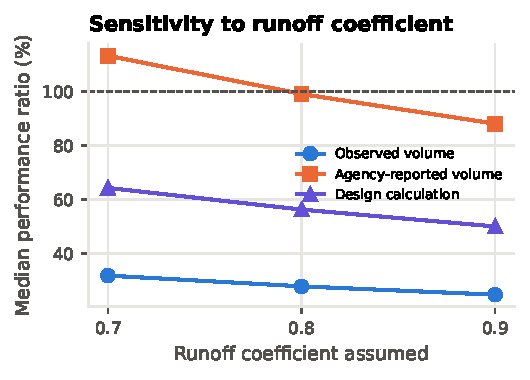
\includegraphics[width=0.46\textwidth]{../figures/figS1_sensitivity_runoff.pdf}\hfill
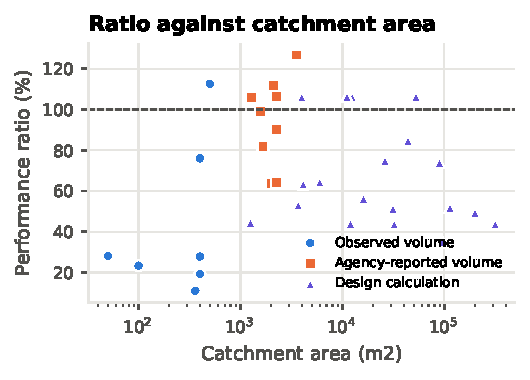
\includegraphics[width=0.46\textwidth]{../figures/figS2_ratio_vs_area.pdf}
\caption{Left: median performance ratio by tier for runoff coefficients 0.70, 0.80 and 0.90. Right: performance ratio against catchment area; the ratio does not rise with size within the observed tier.}\end{figure}

\section{Cost dataset and benchmarks}
\paragraph{Method.} Capital cost in the source's cost year was converted to 2024 rupees with the CPI-IW annual averages (RBI Handbook Table 37; the 1982, 2001 and 2016 base series linked with the published factors 4.63 and 2.88). Annual cost = capital$_{2024}$ $\times$ (CRF + 0.02), where CRF is the capital recovery factor for 15 years at 8\% (0.1168) and 0.02 is the CGWB manual's O\&M norm (2\% of capital per year, Section 9). The 15-year life and the 2\% O\&M share are the manual's norms; the 8\% discount rate is an assumption (a real rate typical for public infrastructure), and the manual's own worked example uses a 15\% rate, which is reported as a sensitivity in Table~\ref{tab:coststats}. Cost per kL = annual cost divided by the annual yield stated by the source. For CSE Delhi projects that yield is already a design share (35 to 85\%) of area $\times$ rainfall; for Shram Shakti Bhawan it is the CGWB design recharge; for the Bhubaneswar HP building it is the mean of three monitored years. The observed-yield case multiplies all costs by the design-calculated median divided by the observed median. This single multiplier is an approximation: individual design shares range from 35 to 85\% of potential, and non-CSE rows state their yield differently, so per-row rescaling would move individual systems but not the median by much. The BEL Bengaluru project (Rs 57 lakh) was excluded because its cost includes a 170 ML surface reservoir, and SV Symphony because its reported volumes are physically implausible for its roof area.
{\scriptsize\setlength{\tabcolsep}{3pt}
\begin{longtable}{l p{3.2cm} p{2.3cm} r r l r p{1.6cm} r r}
\caption{Cost dataset: 27 systems. Capital deflated to 2024 rupees with CPI-IW (RBI Table 37, linked series); levelised cost = capital $\times$ (CRF at 8\%, 15 years + 0.02) / annual yield. The 8\% rate is our assumption; the 15-year life and 2\% O\&M are the CGWB manual's norms and its example uses 15\% (Table~\ref{tab:coststats}). Source URLs and quotes for every row are in the source extraction table supplied with the data.}\label{tab:cost}\\
\toprule
\textbf{No.} & \textbf{Site} & \textbf{Scale / system} & \textbf{Area m$^2$} & \textbf{Capital Rs} & \textbf{Year} & \textbf{Yield kL/yr} & \textbf{Yield basis} & \textbf{Capital 2024 Rs} & \textbf{Rs/kL}\\ \midrule\endfirsthead
\toprule \textbf{No.} & \textbf{Site} & \textbf{Scale / system} & \textbf{Area m$^2$} & \textbf{Capital Rs} & \textbf{Year} & \textbf{Yield kL/yr} & \textbf{Yield basis} & \textbf{Capital 2024 Rs} & \textbf{Rs/kL}\\ \midrule\endhead
\bottomrule\endfoot
1 & Mira Model School, New Delhi & institutional / recharge & 16,200 & 120,000 & 2001 & 4,454 & design & 494,208 & 15.2\\
2 & Janki Devi Memorial College, New Delhi & institutional / recharge & 32,170 & 70,000 & 2001 & 6,880 & design & 288,288 & 5.7\\
3 & Jamia Hamdard University, New Delhi & institutional / recharge & 315,380 & 652,000 & 2001 & 67,444 & design & 2,685,197 & 5.4\\
4 & The Shri Ram School, New Delhi & institutional / both & 6,000 & 125,000 & 2000 & 1,890 & design & 536,809 & 38.9\\
5 & Tex Corp Ltd, Gurgaon & industrial / storage & 4,000 & 550,000 & 2002 & 1,962 & design & 2,175,908 & 151.7\\
6 & Ford Foundation, New Delhi & institutional / recharge & 12,500 & 400,000 & 2000 & 6,492 & design & 1,717,789 & 36.2\\
7 & Sri Aurobindo Ashram, New Delhi & institutional / recharge & 95,870 & 400,000 & 2003 & 16,366 & design & 1,525,475 & 12.8\\
8 & Tihar Jail wards 1 and 13, New Delhi & institutional / recharge & 4,125 & 20,000 & 2002 & 1,280 & design & 79,124 & 8.5\\
9 & Indian Spinal Injury Centre, New Delhi & institutional / recharge & 52,598 & 80,000 & 2002 & 27,317 & design & 316,496 & 1.6\\
10 & BPCL housing complex, Noida & residential colony / recharge & 13,910 & 450,000 & 2002 & 4,446 & design & 1,780,288 & 54.8\\
11 & Defence Colony C block, New Delhi & residential colony / recharge & 26,087 & 258,000 & 2003 & 9,563 & design & 983,931 & 14.1\\
12 & Hero Honda Motors, Daruhera & industrial / recharge & 11,080 & 1,200,000 & 2004 & 5,441 & design & 4,400,392 & 110.7\\
13 & Anup Ahuja farm house, New Delhi & individual house / recharge & 1,250 & 20,000 & 2002 & 272 & design & 79,124 & 39.8\\
14 & Surya Vihar apartments, Gurgaon & residential colony / recharge & 44,029 & 65,000 & 2002 & 18,207 & design & 257,153 & 1.9\\
15 & Mother Dairy unit, New Delhi & industrial / recharge & 89,370 & 435,000 & 2004 & 32,250 & design & 1,595,142 & 6.8\\
16 & New Friends Club, New Delhi & institutional / recharge & 3,700 & 40,000 & 2004 & 961 & design & 146,680 & 20.9\\
17 & Delhi Gymkhana Club, New Delhi & institutional / recharge & 113,344 & 80,000 & 2004 & 28,766 & design & 293,359 & 1.4\\
18 & Nizamuddin East colony, New Delhi & residential colony / recharge & 200,916 & 174,000 & 2004 & 48,531 & design & 638,057 & 1.8\\
19 & Royal Bhutanese Embassy, New Delhi & institutional / recharge & 31,363 & 110,000 & 2004 & 7,867 & design & 403,369 & 7.0\\
20 & Brig. Jagdev Singh residence, New Delhi & individual house / recharge & 285 & 7,500 & 2001 & 147 & design & 30,888 & 28.8\\
21 & Shram Shakti Bhawan, New Delhi & institutional / recharge & 11,965 & 410,000 & 2001 & 3,000 & design & 1,688,544 & 77.0\\
22 & Nandi Deepa apartments, Bengaluru & residential colony / recharge & NR & 2,220,000 & 2021 & 3,564 & design & 2,560,161 & 98.3\\
23 & Vidhani village houses, cluster (Saini et al.), Jaipur & residential colony / storage & 2,466 & 131,498 & 2016 & 1,602 & design & 196,218 & 16.8\\
24 & TSSM BSCOER and JSPM campuses (Varpe et al.), Pune & institutional / both & 8,200 & 6,204,336 & 2019 & 5,453 & design & 7,910,817 & 198.5\\
25 & Bearys modular house system (Raju et al.), Mangaluru & individual house / storage & 81 & 5,710 & 2021 & 21 & design & 6,585 & 43.3\\
26 & Punjab govt building standard design (900 m2) & institutional / recharge & 900 & 281,079 & 2020 & 438 & design & 340,630 & 106.4\\
27 & Hydrology Project building, Bhubaneswar & institutional / recharge & 2,250 & 856,000 & 2004 & 2,279 & agency-monitored, method not stated (mean 2004-06) & 3,138,946 & 188.5\\
\end{longtable}}


\begin{table}[H]\centering\small
\caption{Levelised cost per kL of design yield (2024 rupees) by group, and sensitivity.}\label{tab:coststats}
\begin{tabular}{lrrr}\toprule
Group & n & Median Rs/kL & Range\\ \midrule
All & 27 & 20.9 (95\% CI 8.5--43.3) & IQR 6.9--65.9\\
individual house & 3 & 39.8 & 28.8--43.3\\
residential colony & 6 & 15.4 & 1.8--98.3\\
institutional & 15 & 15.2 & 1.4--198.5\\
industrial & 3 & 110.7 & 6.8--151.7\\
system: recharge & 22 & 14.6 & \\
system: storage & 3 & 43.3 & \\
system: both & 2 & 118.7 & \\
CSE Delhi-NCR rows (2000--2004) & 20 & 13.4 &\\
Rows with cost year $\geq$ 2010 & 5 & 98.3 &\\
Sensitivity: 20-year life, 6\% discount & 27 & 16.4 &\\
Sensitivity: 15\% discount (the CGWB example rate) & 27 & 29.2 &\\
Rows with cost year $\geq$ 2010 at observed yield & 5 & 199 &\\
At observed yield (multiplier 2.02) & 27 & 42 &\\
\bottomrule\end{tabular}
\end{table}
Kruskal-Wallis across the four building-scale groups: H = 2.07, p = 0.559. Spearman $\rho$ of $\log_{10}$ area against Rs/kL: -0.74 (p = 0.0000, n = 26); against capital per m$^2$: -0.73 (p = 0.0000). The delivered-yield multiplier is the design-calculated median ratio (design yield as a share of potential, 0.56) divided by the observed median (0.28).

\begin{figure}[H]\centering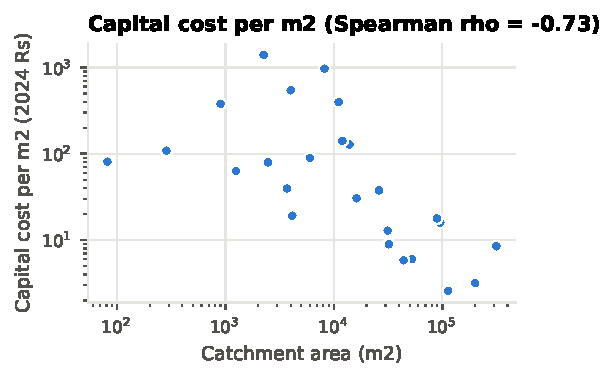
\includegraphics[width=0.5\textwidth]{../figures/figS3_capital_per_m2.pdf}
\caption{Capital cost per m$^2$ of catchment (2024 rupees) against catchment area, 26 systems with a stated area.}\end{figure}
{\tiny\setlength{\tabcolsep}{3pt}
\begin{longtable}{p{4cm} p{1.5cm} p{2.5cm} p{2.1cm} p{1.7cm} p{3.4cm}}
\caption{Price benchmarks collected. The eight used in the cost figure of the main report are the Chennai lowest and top domestic slabs, the Delhi 20--30 kL slab, the BWSSB production cost, Chennai desalination O\&M, the Metrowater 9 kL tanker, and the Bengaluru 2024 and Chennai 2019 private tanker prices (Rs per load divided by load volume).}\label{tab:bench}\\
\toprule
\textbf{Item} & \textbf{City} & \textbf{Value} & \textbf{Unit} & \textbf{Year} & \textbf{URL}\\ \midrule\endfirsthead
\toprule \textbf{Item} & \textbf{City} & \textbf{Value} & \textbf{Unit} & \textbf{Year} & \textbf{URL}\\ \midrule\endhead
\bottomrule\endfoot
CMWSSB domestic metered water tariff, up to 10 kL & Chennai & 7.00 & Rs/kL & 2025 (w.e.f. 01-Apr-2025) & \url{https://www.cmwssb.tn.gov.in/tariff}\\
CMWSSB domestic metered water tariff, above 25 kL & Chennai & 48.00 & Rs/kL & 2025 & \url{https://www.cmwssb.tn.gov.in/tariff}\\
CMWSSB lorry (tanker) water supply, domestic 9,000 L & Chennai & 700 & Rs per 9,000 L load (= Rs 77.8/kL, derived) & 2023/2025 (w.e.f. 01-Apr-2023 and 01-Apr-2025) & \url{https://www.cmwssb.tn.gov.in/tariff}\\
Chennai Metrowater tanker 9,000 L price hike & Chennai & 735 & Rs per 9,000 L load & 2019 (Oct) & \url{https://www.thenewsminute.com/amp/story/tamil-nadu/chennai-metrowater-hikes-tanker-price-without-any-public-announcement-110817}\\
Chennai Metrowater public tanker 9,000 L during 2019 crisis & Chennai & 700 & Rs per 9,000 L load & 2019 (June) & \url{https://www.thenewsminute.com/amp/story/tamil-nadu/chennai-water-crisis-private-tankers-fleece-public-rates-increase-over-100-103859}\\
Chennai private tanker 12,000 L, pre-crisis & Chennai & 1500-2000 & Rs per 12,000 L load & 2018-2019 (April 2019 / 'last June') & \url{https://www.thenewsminute.com/amp/story/tamil-nadu/chennai-water-crisis-private-tankers-fleece-public-rates-increase-over-100-103859}\\
Chennai private tanker 12,000 L, June 2019 crisis peak & Chennai & 3000-6000 & Rs per 12,000 L load & 2019 (May-June) & \url{https://www.thenewsminute.com/amp/story/tamil-nadu/chennai-water-crisis-private-tankers-fleece-public-rates-increase-over-100-103859}\\
Chennai Metrowater tanker 9,000 L (2004) & Chennai & 650 & Rs per 9,000 L load & 2004 & \url{https://www.downtoearth.org.in/amp/story/environment/tanker-economics-12249}\\
Chennai desalination (Minjur/Nemmeli) O\&M cost & Chennai & 68000 & Rs per MLD (= Rs 68/kL, derived) & 2019 & \url{https://citizenmatters.in/chennai-cost-of-desalination-vs-surface-water-treatment-plants-8405}\\
Chennai surface water treatment O\&M cost & Chennai & 6000-23000 (avg 14500) & Rs per MLD (= Rs 6-23/kL, derived) & 2019 & \url{https://citizenmatters.in/chennai-cost-of-desalination-vs-surface-water-treatment-plants-8405}\\
Minjur desalination bulk purchase price paid by Metrowater & Chennai & 48.66 & Rs/kL & 2012 (The Hindu, 19 Apr 2012) / 2010 agreement & \url{https://en.wikipedia.org/wiki/Minjur_Seawater_Desalination_Plant}\\
BWSSB Cauvery water production cost & Bengaluru & 41 & Rs/kL & 2021 & \url{https://citizenmatters.in/rainwater-harvesting-in-bengaluru-webinar-64351}\\
BWSSB domestic tariff revision - increase by slab & Bengaluru & 0.15 paise/L (0-8000 L); 0.30 paise/L (8001-25000 L); 0.80 paise/L (25001-50000 L); 'Re 1 per litre' (>50000 L, likely paise) & increase per litre & 2025 (order 10 Apr 2025, bills from May 2025) & \url{https://www.theweek.in/wire-updates/national/2025/04/09/mes24-ka-water-hike.html}\\
BWSSB minimum domestic slab after April 2025 revision & Bengaluru & 0.30 paise per litre (= Rs 3/kL) & Rs/kL (derived) & 2025 & \url{https://www.etvbharat.com/en/!bharat/bangalore-water-board-revises-tariff-residents-vent-anger-over-extra-burden-enn25041005877}\\
Bengaluru private tanker, pre-crisis vs crisis (resident reports) & Bengaluru & 600-1000 before; 1800-2000 during & Rs per 12,000 L load & 2024 (Feb-Mar) & \url{https://businesstoday.in/india/story/bengaluru-water-crisis-district-administration-fixes-rates-for-water-tanker-services-420502-2024-03-07}\\
Bengaluru district administration capped tanker rates (within 5 km) & Bengaluru & 600 (6,000 L); 700 (8,000 L); 1,000 (12,000 L) & Rs per load, incl GST & 2024 (7 Mar 2024, for 4 months) & \url{https://businesstoday.in/india/story/bengaluru-water-crisis-district-administration-fixes-rates-for-water-tanker-services-420502-2024-03-07}\\
Delhi Jal Board domestic volumetric tariff (Category I) & Delhi & 5.27 (up to 20 kL); 26.36 (20-30 kL); 43.93 (>30 kL) & Rs/kL plus service charge Rs 146.41 / 219.62 / 292.82 per month; sewer charge 60\% of volumetric & NR (Citizen's Charter PDF, undated) & \url{https://delhijalboard.delhi.gov.in/sites/default/files/inline-files/citizen_s_charter.pdf}\\
Delhi private tanker prices (DTE investigation) & Delhi & 2,500 (8,000 L); 5,000 (one full tanker, >=10,000 L) & Rs per load & 2024 (June) & \url{https://www.downtoearth.org.in/amp/story/water/tanker-economy-revealed-dte-uncovers-how-water-suppliers-openly-exploit-the-poor-across-delhi}\\
BMC Mumbai residential piped water tariff & Mumbai & 5.94 (up to 150 lpcd); 11.88 (150-200 lpcd); 17.82 (200-250 lpcd); 23.76 (>250 lpcd) & Rs/kL & 2021 & \url{https://citizenmatters.in/how-much-do-mumbaikars-pay-for-water-28014}\\
HMWSSB domestic tariff (approx., last revision) & Hyderabad & \textasciitilde 10 & Rs/kL & 2026 (article 16 Sep 2026; refers to last revision) & \url{https://www.siasat.com/water-bills-to-rise-by-5-pc-annually-as-hmwssb-looks-to-recover-revenue-3543386/}\\
Hyderabad RWH pit cost (contractor example, HMWSSB mandate) & Hyderabad & 100000-120000 & Rs per pit (6 ft x 6 ft) & 2024 & \url{https://thesouthfirst.com/telangana/hmwssb-mandates-rainwater-harvesting-pits-for-17000-buildings-to-tackle-water-crisis}\\
Recharge structure cost table (CGWB-type norms as reproduced by IIT Bombay) & India (generic) & Recharge pit 2500-5000; Recharge trench 5000-10000; Recharge through hand pump 1500-2500; Recharge through dug well 5000-8000; Recharge well 50000-80000; Recharge shaft 60000-85000; Lateral shaft per m 2000-3000 + bore well 25000-35000 & Rs per structure & NR (lecture undated; CGWB source c.2000s) & \url{https://arctest.dev.nptel.ac.in/content/storage2/courses/105101010/downloads/Lecture11.pdf}\\
CGWB dug well recharge average unit cost (XI Plan scheme) & India (7 states) & 4000 (range 3600-5700) & Rs per dug well recharge structure & 2011 (XI Plan) & \url{https://www.cgwb.gov.in/cgwbpnm/download/379}\\
CSE: RWH cost for existing building of \textasciitilde 300 sq m & Delhi (generic) & 2000-30000 & Rs per system & NR (page undated) & \url{https://www.cseindia.org/costs-1097}\\
CSE unit rates: PVC storage tank & Delhi / Mumbai / Pune / Rajkot / Chennai / Kolkata & 6.00 / 4.25 / 7.00 / 6.00 / 3.00 / 5.4 & Rs per litre of tank capacity & NR (undated) & \url{https://www.cseindia.org/costs-1097}\\
CSE unit rates: recharge bore drilling & Delhi / Mumbai / Pune / Rajkot / Chennai / Kolkata & 600 (hand) / 1000 (mechanical); 10000; 197; 225; 160 (7in); 931 (first 50 m) & Rs per metre & NR (undated) & \url{https://www.cseindia.org/costs-1097}\\
Rain Centre Chennai: sump storage cost & Chennai & 3.5-4 & Rs per litre of storage & NR (c.2003; Rain Centre leaflet) & \url{https://static.vikaspedia.in/media/files_en/energy/environment/three-main-design-concepts.pdf}\\
Rain Centre Chennai: recharge well cost & Chennai & 400 & Rs per foot of depth & 2003 & \url{https://www.indiatogether.org/environment/water/rwh-rkrish-may03.pdf}\\
Rainwater Club Bengaluru: ferrocement tank unit cost & Bengaluru & 1.20 & Rs per litre of storage & NR (undated) & \url{https://Sswm.info/sites/default/files/reference_attachments/RAINWATERCLUB%20Editor%20ny%20Rooftop%20Rainwater%20Harvesting%20for%20tackling%20Fluoride%20contaminated%20Ground%20Water.pdf}\\
Typical Chennai house RWH retrofit cost (1000-1200 sq ft terrace) & Chennai & 5000-8000 & Rs per house & 2017 & \url{https://citizenmatters.in/how-to-start-harvesting-rainwater-at-home-3181}\\
Residential RWH with 10,000 L storage (Organiser op-ed) & India (generic) & 20000 & Rs per system; storage Rs 1.5-2 per litre & 2009 & \url{https://organiser.org/2009/10/04/38978/general/r1419f082/}\\
O\&M cost statement - secondary guide (Studio Matrx) & India (generic) & 2000-5000 & Rs per year & 2026 & \url{https://www.studiomatrx.org/guides/rainwater-harvesting}\\
O\&M cost statement - secondary guide (Houseyog) & India (generic) & 2000-5000 & Rs per year & 2025/2026 & \url{https://www.houseyog.com/blog/rainwater-harvesting-cost-india/}\\
O\&M cost statement - vendor (NeeRain) & India (generic) & 0-500 & Rs per year & 2026 & \url{https://neerain.com/rooftop-rainwater-harvesting-real-cost/}\\
O\&M frequency statements (CSE) & India (generic) & NR & frequency only & NR & \url{https://www.cseindia.org/maintenance-monitoring-1125}\\
Payback statement - campus RWH + reclamation (peer-reviewed) & India (hot semi-arid campus) & >250 & years payback & 2020 & \url{https://eprints.ncl.ac.uk/271510}\\
Private tanker cost assumption used in Pune campus payback calc & Pune & 1560000 & Rs per year (campus tanker expenditure) & 2019 & \url{http://www.ijirset.com/upload/2019/june/43_Rooftop.pdf}\\
\end{longtable}}


\section{Functionality, installation and failure modes}
{\scriptsize\setlength{\tabcolsep}{3pt}
\begin{longtable}{l p{2.8cm} p{2.6cm} r r p{4.6cm} p{2.9cm}}
\caption{Functional-share estimates: 13 estimates from 12 surveys (the two Dwarka rows are two definitions applied to one DJB report). URLs and quotes are in the source extraction table supplied with the data.}\label{tab:func}\\
\toprule
\textbf{No.} & \textbf{Survey} & \textbf{Population} & \textbf{n} & \textbf{Functional \%} & \textbf{Definition used} & \textbf{Conducted by (reported via)}\\ \midrule\endfirsthead
\toprule \textbf{No.} & \textbf{Survey} & \textbf{Population} & \textbf{n} & \textbf{Functional \%} & \textbf{Definition used} & \textbf{Conducted by (reported via)}\\ \midrule\endhead
\bottomrule\endfoot
1 & Chennai 2019, houses with a structure & houses with an RWH structure (1.62 lakh of 2.72 lakh inspected) & 162,000 & 76 & 1.62 lakh houses had a structure; about 38,000 of them 'needed minor repairs', so 1.24 lakh (76.5\%) needed no repair. Single GCC snapshot (Aug-Sep 2019). & Greater Chennai Corporation (The News Minute)\\
2 & Chennai Gandhinagar 2003 & independent houses & 309 & 50 & 'only 50 per cent had implemented RWH properly' & Akashganga Trust (Down To Earth 2004)\\
3 & Chennai approved buildings 2001-02 & buildings approved under 1994 rule, with RWH & 25 & 67 & a third of installed systems 'not properly designed and therefore ineffective' & MIDS survey for CSE\\
4 & Karnataka school structures 2007 & government school rooftop structures & 1,269 & 11 & 140 of 1,269 structures functional & Arghyam status report\\
5 & Karnataka model schools 2009 & school rooftop structures & 27 & 59 & 16 of 27 functioning; 3 partial; 8 defunct & Arghyam\\
6 & Faridabad public systems 2018-19 & public RWH systems (parks, schools) & 190 & 20 & 'around 80\% had stopped working' & MCF survey (The Tribune)\\
7 & Faridabad public systems 2024 & public RWH systems & 200 & 25 & 'around 70 to 80 per cent' non-functional (midpoint) & civic sources (The Tribune)\\
8 & Gurugram pits 2023 & RWH pits, public and private & 500 & 30 & 'around 70\%' lying defunct & MCG / GMDA (The Tribune)\\
9 & Delhi Dwarka societies 2024 (structural) & group housing societies with RWH & 176 & 84 & 176 minus 4 non-functional minus 25 dry pits & DJB action-taken report to NGT\\
10 & Delhi Dwarka societies 2024 (clean recharge) & group housing societies with RWH & 176 & 32 & 57 of 176 without faecal coliform in recharge water (119 contaminated) & DJB action-taken report to NGT\\
11 & Bengaluru BWSSB connections 2023 (expert estimate) & BWSSB connections with RWH & NR & 40 & 'only about 40\% of BWSSB connections have functional RWH systems' (estimate) & S. Vishwanath (Deccan Herald)\\
12 & Kaithal government buildings 2018 & government-building systems & 5 & 0 & all five choked after the first year & The Tribune field report\\
13 & Sirsa park systems 2025 & municipal park systems & 4 & 50 & 2 of 4 dead within two years & The Tribune field report\\
\end{longtable}}

\paragraph{Notes on the Chennai 2019 figures.} The Tamil Nadu government and the Greater Chennai Corporation reported the 2019 inspection drive in two snapshots: over 2 lakh buildings (1.36 lakh correctly installed and maintained, 37,131 needing maintenance, 60,461 without a structure) and, a few weeks later, about 2.72 lakh houses (1.62 lakh with a structure, about 38,000 of them needing minor repairs, almost 70,000 without). To avoid mixing snapshots, both steps of the Chennai cascade use the second one: 1.62 of 2.72 lakh houses had a structure (59.6\%) and 1.24 of 1.62 lakh needed no repair (76.5\%). The first snapshot gives a similar functional share (1.36 of 1.73 lakh, 78.6\%). Both reach us through press reports (The News Minute); no original press release was located.
{\scriptsize\setlength{\tabcolsep}{3pt}
\begin{longtable}{p{2.5cm} p{3.4cm} r r r p{5.5cm}}
\caption{Installation (compliance) figures used in the mandate-gap figure of the main report.}\label{tab:compl}\\
\toprule
\textbf{City} & \textbf{Population} & \textbf{Denominator} & \textbf{With RWH} & \textbf{\%} & \textbf{Definition}\\ \midrule\endfirsthead
\toprule \textbf{City} & \textbf{Population} & \textbf{Denominator} & \textbf{With RWH} & \textbf{\%} & \textbf{Definition}\\ \midrule\endhead
\bottomrule\endfoot
Chennai 2019 & houses inspected & 272,000 & 162,000 & 59.6 & 1.62 lakh of 2.72 lakh inspected had a structure\\
Bengaluru 2023 & properties with water connection & 1,080,000 & 190,000 & 17.6 & 1.9 lakh of 10.8 lakh\\
Hyderabad 2024 & properties >= 300 sq yd surveyed & 39,000 & 22,000 & 56.4 & 22,000 installed; 17,000 non-compliant\\
Mumbai 2007-21 & housing societies (estimate) & 20,000 & 3,000 & 15.0 & about 3,000 of about 20,000 societies\\
Pune FY2022-23 & taxable properties (rebate claimants) & 1,250,000 & 3,716 & 0.3 & 3,716 rebate claimants of about 12.5 lakh properties\\
Nagpur 2023 & properties & 636,000 & 1,123 & 0.2 & 1,123 of about 6.36 lakh properties\\
Delhi govt buildings 2019 & government buildings (building class, not a city rate) & 771 & 212 & 27.5 & 212 of 771 with RWH\\
\end{longtable}}

{\scriptsize\setlength{\tabcolsep}{3pt}
\begin{longtable}{p{5cm} r r p{7.5cm}}
\caption{Failure-mode categories (11 after collapsing), number of distinct sources citing each (90 mentions from 40 distinct sources; these overlap with but are not the same set as the 46 survey records), and the cities concerned. Every mention with URL and quote is in the source extraction table supplied with the data.}\label{tab:fm}\\
\toprule
\textbf{Failure mode} & \textbf{Sources} & \textbf{Mentions} & \textbf{Cities}\\ \midrule\endfirsthead
\toprule \textbf{Failure mode} & \textbf{Sources} & \textbf{Mentions} & \textbf{Cities}\\ \midrule\endhead
\bottomrule\endfoot
No maintenance, abandoned & 18 & 18 & Bengaluru, Chennai, Delhi, Delhi (Dwarka), Delhi (school), Delhi schools, Faridabad, Gurugram, Hyderabad, Karnataka schools\\
No awareness, incentive or enforcement & 15 & 15 & Bengaluru, Chennai, Delhi, Faridabad, Karnataka schools, Mumbai\\
Poor design or construction & 15 & 17 & Bengaluru, Chennai, Delhi, Delhi (Dwarka), Faridabad, Karnataka schools, Mumbai, Sirsa\\
Token structure, built for compliance only & 10 & 10 & Bengaluru, Chennai, Gurugram, Mumbai, Thane\\
Recharge pit or well silted or choked & 7 & 7 & Chennai, Delhi, Delhi (Dwarka), Faridabad, Kaithal\\
Downpipes or conveyance broken or disconnected & 6 & 6 & Bengaluru, Chennai, Delhi schools, Karnataka schools\\
Other (space, vandalism, roof-only design) & 6 & 7 & Bengaluru, Chennai, Delhi, Karnataka schools\\
Storage undersized, overflow or leak & 3 & 3 & Bengaluru, Karnataka schools, Mumbai\\
Filter clogged or absent & 3 & 3 & Bengaluru, Chennai, Karnataka schools\\
First flush absent or not operated & 2 & 2 & Delhi, Karnataka schools\\
Water quality concerns, system disused & 2 & 2 & Delhi (Dwarka), Karnataka schools\\
\end{longtable}}

\paragraph{Outcome evidence.} The often-quoted 6 to 8 m rise in Chennai groundwater after 2003 traces only to the Rain Centre's own statements; the CMWSSB figure of a 4 m net rise and The Hindu's 2006 report of a 2 m monsoon rise are not attributed to rooftop RWH specifically. In 2019 the Rain Centre reported 90\% of its 88 monitoring wells dry despite 16 years of the mandate. BWSSB data suggest about 10\% of Bengaluru's runoff is harvested, around 3\% of demand. Delhi Jal Board paid Rs 325.7 million in RWH rebates and collected Rs 567.1 million in penalties between 2017 and 2019 (details and URLs in the functionality search log supplied with the data).

\section{Mandate instruments and reference inputs}
{\tiny\setlength{\tabcolsep}{3pt}
\begin{longtable}{p{2.1cm} p{3cm} p{1.3cm} p{3cm} p{2.9cm} p{3.4cm}}
\caption{Mandate landscape, 24 jurisdictions. URLs and quotes are in the source extraction table supplied with the data.}\label{tab:mandates}\\
\toprule
\textbf{Jurisdiction} & \textbf{Instrument} & \textbf{Year} & \textbf{Applies to} & \textbf{Penalty / incentive} & \textbf{Reported compliance}\\ \midrule\endfirsthead
\toprule \textbf{Jurisdiction} & \textbf{Instrument} & \textbf{Year} & \textbf{Applies to} & \textbf{Penalty / incentive} & \textbf{Reported compliance}\\ \midrule\endhead
\bottomrule\endfoot
India (Model Building Bye-Laws 2016, MoHUA) & Model Building Bye-Laws 2016 (MBBL), MoHUA; rainwater harvesting chapter & 2016 & all buildings having a plot size of 100 sq.m or more (RWH proposal required with building plan) & NR (states decide) & 33 States/UTs have adopted the RWH provisions (Lok Sabha reply 05.03.2020; also PIB 24.03.2020); 'barring Sikkim, Lakshadweep and Mizoram' all States/UTs adopted (Lok Sabha Q1241, 09.02.2023)\\
Tamil Nadu (incl. Chennai) & Tamil Nadu Municipal Laws (Second Amendment) Ordinance, 2003 (TN Ordinance No. 4 of 2003) inserting s.255-A Chennai City Municipal Corporation Act etc. & 2003 (promulgated 19 July 2003) & every owner or occupier of a building (all buildings; Govt buildings too) & water supply connection disconnected until structure provided; Commissioner may build and recover cost as property tax; new buildings not given water/sewer connection without RWH (CSE) & Chennai 2019: GCC inspected \textasciitilde 2.72 lakh houses since Aug 2019, \textasciitilde 1.62 lakh had RWH (approx 60\%), 9,000 notices issued; CMWSSB claims 8.9 lakh structures; Rain Centre 2015 audit of 1,100 samples found govt buildings worst violators\\
Bengaluru (BWSSB jurisdiction) & Bangalore Water Supply and Sewerage (Amendment) Act, 2011 (Karnataka Act No. 05 of 2011) substituting s.72A (bill introduced 2009); penalty regulations 2015; BWSS (Amendment) Bill 2021 extends to 30x40 sites & 2009 (bill) / 2011 (Act assented 2 Feb 2011) / 2021 (extension) & existing buildings on sital area >= 2400 sq ft (60x40 ft site); new buildings on sital area >= 1200 sq ft (30x40 ft); 2021 Bill: sital area 2,325-10,763.9 sq ft RWH; >=10,763.9 sq ft dual piping + RWH & residential: 25\% of water bill first 3 months then 50\%; non-residential: 50\% then 100\% (Citizen Matters 2023); Rs 1.95-2 crore/month collected & Dec 2023: \textasciitilde 1.9 lakh of 10.8 lakh properties with water connections (\textasciitilde 18\%) have RWH; 39,703 properties paying monthly penalty; Mar 2024 (The Hindu): 1,96,591 residential buildings implemented, 39,213 have not\\
Karnataka (statewide, outside BWSSB) & Government orders for Government buildings; statewide urban mandate 'contemplated' (2011); 20\% tax rebate (CSE) & NR & Government buildings; amendment of bye-laws in cities >20 lakh population under action (CSE); statewide new buildings contemplated 2011 & 20\% rebate on tax payment for 5 years (CSE) & NR\\
Delhi (NCT) & Building Bye-laws 1983 modified by MoUD Gazette Notification 28.07.2001 (plots >=100 sq m); CGWA directive; DJB resolution No. 829; Unified Building Bye-Laws 2016 & 2001 (bye-law), 2012 (DJB mandatory per Outlook), 2016 (UBBL) & all buildings with plot area >= 100 sq m (2001 notification; DJB resolution 829); DJB compulsory for plots >= 500 sq m; UBBL 2016 features mandatory for new constructions above 105 sq m (DUAC) & building plans not sanctioned without RWH; DJB 10\% rebate on water bill for plots >= 100 sq m with functional RWH; penalty 1.5 times water bill / '50\% of the monthly bill amount' for non-compliance; proposed environmental compensation Rs 50,000 to Rs 5 lakh (2023 proposal); NGT Rs 5 lakh per educational institution (OA 217/2016) & Delhi: 1,560 consumers availed DJB rebate (NGT monitoring committee report OA 496/2016); 3,675 govt schools/colleges of 4,769 institutions had functional systems; only 1,869 private buildings as of 2021 (Citizen Matters); Dwarka: NGT expert committee inspected 354 CGHS, 'Most structures are found either completely defunct or just partially working' (2023)\\
Mumbai / Maharashtra (Greater Mumbai DCR; all towns non-gaothan) & Govt of Maharashtra UDD Notification No. TPB-4307/396/CR-124/2007/UD-11 dated 6 June 2007 modifying Development Control Regulations for Greater Mumbai 1991; BMC mandatory for new buildings since 2002 (Citizen Matters); Aug 2026 GR: old buildings seeking new water/drainage connections must have RWH & 2002 (BMC, new buildings) / 2007 (300 sq m notification) & plots having area not less than 300 sq m in non-gaothan areas of all towns (2007); earlier 1,000 sq m (CSE) & no building permission unless provision for RWH; levy not exceeding Rs 1000 per annum per 100 sq m built-up area for failure to provide/maintain; completion/occupation certificate only after RWH (CSE) & approx. 3,000 societies of an estimated 20,000 had RWH 2007-2021 (Citizen Matters Jul 2024)\\
Hyderabad / Telangana (HMWSSB area) & AP Govt order (2000) for all municipal corporations/urban areas (IWP); APWALTA 2002; HMWSSB directive dated 14 Dec 2024 for 17,000 consumers & 2000 (GO; tentative enforcement June 2001) & all new buildings with area 300 sq m or more irrespective of roof area; existing buildings within one year of GO (CSE); originally 200 sq m then 300 sq m (Realty Today) & 50\% subsidy on RWH structures was lifted due to poor response (CSE); 2024: double charges for HMWSSB water tankers for non-compliant (Rs 500 to Rs 1,000 per 5 kL) & Dec 2024: NGO survey of 39,000 properties; 42,000 buildings identified needing RWH; 22,000 installed; 17,000 non-compliant (Realty Today / South First)\\
Pune (PMC) & PMC requirement for new buildings (2006, per Realty Today); property-tax rebate scheme & 2006 & all new buildings (Realty Today) & property tax rebate up to 10\% for RWH (PMC eco-housing rebate) & 306 properties availed rebate in FY2012-13; 3,716 in FY2022-23, of approx. 12.5 lakh taxable properties (approx 0.3\%)\\
Nagpur (NMC) & NMC regulation (mandatory from March 2005 per CSE; ruling effective 28 Aug 2009 per Propnewstime) & 2005 (CSE) / 2009 (Propnewstime) & new constructions of area >= 300 sq m (non-gaothan); housing society layouts and amenity spaces & fine up to Rs 1,000 per annum per 100 sq m built-up area; NMC 5-10\% property tax discount for eco initiatives & May 2023: only 1,123 buildings comply = 0.18\% of \textasciitilde 6.36 lakh properties\\
Gujarat / Ahmedabad (AUDA/AMC GDCR) & Gujarat Development Control Regulations (GDCR); AUDA notification 2002 (1,500 sq m+); State Govt buildings after 2003 & 2002 (AUDA) / 2003 (Govt buildings) & GDCR: buildings 500-1,500 sq m follow RWH specifications; 1,500-4,000 sq m percolation wells (one per 4,000 sq m); AUDA 2002: constructions >= 1,500 sq m & Surat: 50\% subsidy up to Rs 2,000 (CSE); no penalty stated & NR ('still not very popular', 2008 clipping)\\
Rajasthan / Jaipur (JDA) & Rajasthan state mandate (PHED certification); Jaipur/Rajasthan Building Bye-Laws 2020 Regulation 21.7 (rule 10.11.1); JDA enforcement 2011 & 2011 (JDA penalty) / 2020 (Bye-laws) & all buildings (any land use) with plot area over approx. 300 sq m (CSE legislation page) / over 500 sq m (CSE laws page); Bye-laws 2020: each plot owner (no minimum stated in translation) & water supply connection can be terminated if RWH completion certificate not submitted to PHED; JDA penalty Rs 25,000 (2011); Bye-laws 2020: annual maintenance fee levied by local authority & Jul 2023: only 220 buildings in Jaipur had complied (JDA)\\
Madhya Pradesh / Indore (also Jabalpur, Gwalior) & MP Government Order no. F 23 (107) 95 XXXII dated 7 July 2004; MP Bhumi Vikas Rules 1984; Jabalpur from 1 Apr 2005; Gwalior order 27 Jan 2006 & 2004 & all new buildings with area >= 250 sq m; mandatory for G+3 structures & 6\% property tax rebate; Gwalior penalty Rs 7,000 for non-compliance & NR\\
Kerala & Kerala Municipality Building (Amendment) Rules, 2004 (Extraordinary Gazette No. 92/2004 dated 12-01-2004) inserting Chapter XVI-A, Rule 109A & 2004 & all new buildings: Residential A1 with floor area >= 100 sq m and plot area >= 200 sq m; A2, B, C, D, E and specified G1/G2 occupancies & no penalty stated; exemption where water logging common; KWA 90\% / Jalanidhi 75\% subsidies (CSE) & NR (CSE: flats with multiple owners maintained better than individual houses)\\
Haryana (incl. Gurugram, Faridabad) & HUDA rules (CSE); Haryana Building Code 2017 & 2017 (Code) & roof rainwater harvesting where rooftop area >= 100 sq m; recharge for Group Housing with plot > 500 sq m (Tribune); HUDA: all new buildings irrespective of roof area (CSE) & NR & Faridabad: MCF survey 2018-19 found \textasciitilde 75-80\% of RWH systems defunct (Tribune Dec 2023)\\
Uttar Pradesh (Kanpur; Ghaziabad; statewide CM direction 2025) & Building bye-laws (Kanpur: >=1000 sq m per CSE legislation page / >=500 sq m per CSE laws page); Ghaziabad bye-laws >=300 sq m; CM direction 4 Oct 2025 for buildings >100 sq m & NR (bye-laws); 2025 (CM order) & Kanpur: new buildings >= 1000 sq m (or 500 sq m); Ghaziabad: plots >= 300 sq m; CM 2025: buildings larger than 100 sq m, urban and rural & Ghaziabad: penalties up to Rs 3 lakh depending on plot size and severity (2025) & Ghaziabad: of 100 identified locations, 20 visited (Jul 2025); no counts\\
Punjab (incl. Ludhiana) & Punjab building bylaws notified 2018 (Tribune): RWH for structures > 119 sq yards (earlier 250 sq yd residential / 500 sq yd commercial); RWH Cell in each ULB & 2018 & structures (residential, commercial, institutional) on more than 119 sq yards (approx 100 sq m); earlier residential > 250 sq yd and commercial > 500 sq yd & utility connections denied without RWH and completion certificate (Tribune Bathinda) & NR ('only several property owners ensured proper installation and functioning')\\
Chandigarh (UT) & Chandigarh Administration order (2008) for plots of one kanal or more; CSE: all new buildings & 2008 & plots of one kanal (approx 500 sq yd / 418 sq m) or more; administration mulling lower threshold (2019) & NR (no penalty stated; 'absence of any mechanism to keep a check') & 'only a handful of private building owners complying with it' (Pioneer 2019)\\
West Bengal / Kolkata & West Bengal Municipal (Building) Rules, 2007, Rule 171 & 2007 & NR (threshold not stated in source) & NR & NR\\
Goa & Policy on Rainwater Harvesting, Govt of Goa (15/10/2008, WRD); RWH policy notified in gazette Dec 2022 with plot thresholds (Propnewstime) & 2008 (policy) / 2022 (gazette policy) & 2022 policy: residential complexes/apartments on plots >= 2,000 sq m; commercial complexes >= 1,500 sq m; industrial units >= 10,000 sq m; all government buildings; exempt if STP/greywater recycling exists; 2008: PWD govt buildings (CSE) & NR & NR\\
Himachal Pradesh & State direction: no building plan approved in urban areas without RWH (CSE) & NR & all buildings to be constructed in urban areas; schools, government buildings, rest houses, industries, bus stands & building plan not approved without RWH system & NR\\
Uttarakhand (Mussoorie-Dehradun Development Authority) & MDDA building byelaws provision (CSE); MDDA mandatory for new houses of 1,200 sq ft (Tribune 2011) & NR & all new houses of 1,200 sq ft (Tribune, Mussoorie) & NR & Mussoorie 2011: 'only 30\% hoteliers have adopted roof-top rain water harvesting'\\
Andhra Pradesh (all municipal corporations/urban areas; Visakhapatnam) & AP Government Order (2000) making RWH mandatory in all municipal corporations, UDAs and municipalities; APWALTA 2002 & 2000 & buildings of 300 sq m or more & NR & NR (no Visakhapatnam-specific data found)\\
Rajkot (Gujarat) & Rajkot General Development Control Regulations, Regulation No. 17.18 & NR & buildings with built-up area >= 80 sq m; existing buildings > 1,000 sq m five-year moratorium & NR & NR\\
Ranchi (Jharkhand) & Ranchi Regional Development Authority byelaws & NR & NR & NR & NR\\
\end{longtable}}

{\scriptsize\setlength{\tabcolsep}{3pt}
\begin{longtable}{p{4.8cm} p{2.3cm} p{1.4cm} p{2.1cm} p{5.2cm}}
\caption{Runoff coefficients and rainfall normals used. The CGWB (2007) Table 7.2 values were verified directly in the manual.}\label{tab:refinputs}\\
\toprule
\textbf{Item} & \textbf{Value} & \textbf{Unit} & \textbf{Period} & \textbf{Source document}\\ \midrule\endfirsthead
\toprule \textbf{Item} & \textbf{Value} & \textbf{Unit} & \textbf{Period} & \textbf{Source document}\\ \midrule\endhead
\bottomrule\endfoot
Runoff coefficient - GI sheet roof & 0.9 & coefficient & CGWB 2007 (cited) & Table 7.2 'Runoff Coefficients of Common Types of Roofs', CGWB Manual on Artificial Recharge of Ground Water (2007), as reproduced in Journal of Rural Development 37(2), 2018 (NIRD\&PR)\\
Runoff coefficient - Asbestos roof & 0.8 & coefficient & CGWB 2007 (cited) & same as above\\
Runoff coefficient - Tiled roof & 0.75 & coefficient & CGWB 2007 (cited) & same as above\\
Runoff coefficient - Concrete (RCC) roof & 0.7 & coefficient & CGWB 2007 (cited) & same as above\\
Runoff coefficient - Asphalt or concrete pavement & 0.85 & coefficient & 2007 & Table 4.4 'Usual Values of Runoff Coefficients (K)', Section 4.2.2.1.2, p.25, CGWB Manual on Artificial Recharge of Ground Water (Sept 2007) (fetched directly from cgwb.gov.in)\\
Runoff coefficient - Roof top (range) & 0.75 - 0.95 & coefficient & 2020 & 'Catch the Rain - through Rain Water Harvesting', M.K. Garg, Scientist D, CGWB Faridabad (NWM/NYKS orientation ppt, 10 Dec 2020)\\
Runoff coefficient - Paved area (range) & 0.50 - 0.85 & coefficient & 2020 & same CGWB/NWM ppt\\
Runoff coefficient - Bare ground / unpaved (range) & 0.10 - 0.20 & coefficient & 2020 & same CGWB/NWM ppt\\
Runoff coefficient - Green area (range) & 0.05 - 0.10 & coefficient & 2020 & same CGWB/NWM ppt\\
Runoff coefficient - roof (worked example) & 0.8 & coefficient & 2019 & Down To Earth, 'Catch water where it falls: urban rainwater harvesting', 3 Jul 2019\\
Normal annual rainfall - Chennai (Nungambakkam) & 1376.8 & mm & 1991-2020 & IMD RMC Chennai climatological table\\
Normal annual rainfall - Bengaluru City & 1077.6 & mm & 1991-2020 & IMD Met Centre Bengaluru climatological table\\
Normal annual rainfall - New Delhi (Safdarjung) & 762.3 & mm & 1991-2020 & IMD RMC New Delhi climatological table\\
Normal annual rainfall - Mumbai (Santacruz) & 2502.3 & mm & 1991-2020 & IMD city.imd.gov.in Climatological Table (station id 43003 = Mumbai-Santacruz)\\
Normal annual rainfall - Hyderabad & 859.6 & mm & 1991-2020 & IMD city.imd.gov.in Climatological Table\\
Normal annual rainfall - Pune (Shivajinagar) & 841.2 & mm & 1991-2020 & IMD city.imd.gov.in Climatological Table (station id 43063 = Pune-Shivajinagar)\\
Normal annual rainfall - Nagpur (Sonegaon Airport) & 1151.2 & mm & 1991-2020 & IMD city.imd.gov.in Climatological Table (station id 42867 = Nagpur-Sonegaon)\\
Normal annual rainfall - Nagpur district (range) & 1000-1200 & mm & 1901-1992 & CGWB Ground Water Information, Nagpur District, Maharashtra (1770/DBR/2013), CGWB Central Region Nagpur\\
Average annual rainfall - Ramtek taluka (Nagpur district) & 1043.7 & mm & 2002-2011 average & CGWB Ground Water Information, Nagpur District (2013), Table 3 Rainfall data\\
Normal annual rainfall - Panaji / Goa & 2918.0 & mm & 1981-2010 & IMD city.imd.gov.in Climatological Table (Panjim)\\
Normal annual rainfall - Chandigarh & NR & mm & NR & Not found on an official page (IMD Chandigarh pages give only monthly/seasonal normals)\\
Normal annual rainfall - Jodhpur & 374.3 & mm & 1981-2010 & IMD city.imd.gov.in Climatological Table\\
Normal annual rainfall - Ludhiana & NR & mm & NR & Not found on an official page\\
Normal annual rainfall - Patiala (nearest IMD table to Ludhiana/Chandigarh found) & 875.6 & mm & 1991-2020 & IMD city.imd.gov.in Climatological Table (station id 42101 = Patiala)\\
Normal annual rainfall - Ahmedabad & 824 & mm & 2010-2019 & IMD Met Centre Ahmedabad 'climate' note\\
Normal annual rainfall - Jaipur & 600.3 & mm & 1991-2020 & IMD Met Centre Jaipur climatological table\\
Normal annual rainfall - Kolkata (Alipore) & 1813.3 & mm & 1991-2020 & IMD city.imd.gov.in Climatological Table\\
Normal annual rainfall - Thiruvananthapuram & 1835.3 & mm & 1991-2020 & IMD city.imd.gov.in Climatological Table\\
Normal annual rainfall - Indore & 955.1 & mm & 1991-2020 & IMD city.imd.gov.in Climatological Table (station id 42754 = Indore)\\
Normal annual rainfall - Lucknow & 990.1 & mm & 1971-2000 & IMD Met Centre Lucknow 'Climatology of Lucknow' Table 3\\
Normal annual rainfall - Dehradun & 2161.5 & mm & 1991-2020 & IMD Met Centre Dehradun climatological table\\
Normal annual rainfall - Guwahati & 1695.3 & mm & 1991-2020 & IMD city.imd.gov.in Climatological Table (station id 42410 = Guwahati)\\
Normal annual rainfall - Coimbatore & 618.5 & mm & 1991-2020 & IMD RMC Chennai climatological table\\
Normal annual rainfall - Madurai Airport & 843.3 & mm & 1991-2020 & IMD RMC Chennai climatological table\\
Normal annual rainfall - Visakhapatnam & 1113.1 & mm & 1991-2020 & IMD city.imd.gov.in Climatological Table\\
Normal annual rainfall - Amravati district (for Warud) & 886.4 & mm & NR (IMD normal; period not stated; monthly chart period 1941-1990) & Model Agriculture Contingency Plan (Rainfed), Amravati district, ICAR-CRIDA / PDKV Akola, Section 1.2 Rainfall, 'Source: IMD'\\
Normal annual rainfall - Kochi & 3014.8 & mm & 1981-2010 & IMD city.imd.gov.in Climatological Table\\
\end{longtable}}


\section{Sources}
{\tiny\setlength{\tabcolsep}{3pt}
\begin{longtable}{p{9.2cm} p{2.5cm} p{4.2cm}}
\caption{All 168 distinct source URLs used, with the strand and the first record each supports.}\label{tab:sources}\\
\toprule
\textbf{URL} & \textbf{Strand} & \textbf{First use}\\ \midrule\endfirsthead
\toprule \textbf{URL} & \textbf{Strand} & \textbf{First use}\\ \midrule\endhead
\bottomrule\endfoot
\url{http://www.ijirset.com/upload/2019/june/43_Rooftop.pdf} & Cost & TSSM BSCOER \& JSPM NTC campuses, Narhe (Varpe et al.)\\
\url{https://Sswm.info/sites/default/files/reference_attachments/RAINWATERCLUB%20Editor%20ny%20Rooftop%20Rainwater%20Harvesting%20for%20tackling%20Fluoride%20contaminated%20Ground%20Water.pdf} & Cost & Rainwater Club ASHRAYA small house model (ferrocement tank)\\
\url{https://admin.indiawaterportal.org/articles/rainwater-harvesting-made-mandatory-andhra-pradesh-all-municipal-corporations-and-urban} & Mandates & Hyderabad / Telangana (HMWSSB area)\\
\url{https://admin.indiawaterportal.org/sites/default/files/iwp2/Model_School_Report_Suvarna_Jala__Arghyam_2009.pdf} & Functionality & Arghyam\\
\url{https://admin.indiawaterportal.org/sites/default/files/iwp2/rainwater_harvesting_for_aquifer_storage_recovery.pdf} & Performance & Goa University rooftop RWH + recharge bore well (Case study \\
\url{https://agris.fao.org/search/en/records/65df11d2b766d82b1800245a} & Performance & TNAU Coimbatore SWCE workshop roof (Ray et al. 2014, J Progr\\
\url{https://arctest.dev.nptel.ac.in/content/storage2/courses/105101010/downloads/Lecture11.pdf} & Performance & Shram Shakti Bhawan, New Delhi rooftop/pavement recharge (CG\\
\url{https://base.ac.in/wp-content/uploads/2021/11/BASE-University-WP-Series-12-2021.pdf} & Functionality & BASE University WP 12/2021 (Harshita Bhat, Pleasa Serin Abra\\
\url{https://businesstoday.in/india/story/bengaluru-water-crisis-district-administration-fixes-rates-for-water-tanker-services-420502-2024-03-07} & Benchmarks & Bengaluru private tanker, pre-crisis vs crisis (resident rep\\
\url{https://cag.gov.in/uploads/download_audit_report/2019/Report_no_3_of_2019_Social_General_and_Economic_Sector_(Non_PSU)_Government_of_Haryana.pdf} & Functionality & CAG performance audit\\
\url{https://cdn.cseindia.org/userfiles/Urban%20Rainwater%20harvesting%20report.pdf} & Performance & Goa University rooftop RWH + recharge bore well (Case study \\
\url{https://citizenmatters.in/bengaluru-outer-ring-road-apartment-water-scarcity-bill-solution-rainwater-harvesting-monsoon-44485} & Cost & The Greens, Doddanekundi (ORR)\\
\url{https://citizenmatters.in/bengaluru-rainwater-harvesting-3-lakh-annual-savings-borewell-recharge-37514} & Performance & SV Symphony apartments, Chikkabellandur (Sarjapur Rd)\\
\url{https://citizenmatters.in/bengaluru-rainwater-harvesting-bwssb-kscst-water-36374} & Functionality & BWSSB data (Citizen Matters)\\
\url{https://citizenmatters.in/bengaluru-rwh-plans-problems-solutions/} & Functionality & BWSSB count as quoted by S Vishwanath (Biome) in Citizen Mat\\
\url{https://citizenmatters.in/chennai-cost-of-desalination-vs-surface-water-treatment-plants-8405} & Benchmarks & Chennai desalination (Minjur/Nemmeli) O\&M cost\\
\url{https://citizenmatters.in/chennai-household-rainwater-harvesting-guidelines-3059} & Functionality & Akash Ganga Trust (Sekhar Raghavan, Rain Centre) for CMDA - \\
\url{https://citizenmatters.in/chennai-rainwater-harvesting-infrastructure-government-buildings-2909} & Functionality & Public Works Department (PWD), Tamil Nadu\\
\url{https://citizenmatters.in/how-much-do-mumbaikars-pay-for-water-28014} & Benchmarks & BMC Mumbai residential piped water tariff\\
\url{https://citizenmatters.in/how-to-start-harvesting-rainwater-at-home-3181} & Benchmarks & Typical Chennai house RWH retrofit cost (1000-1200 sq ft ter\\
\url{https://citizenmatters.in/mumbai-rainwater-harvesting-lags-behind/} & Functionality & Indian Express report quoted by Citizen Matters\\
\url{https://citizenmatters.in/rainwater-harvesting-delhi-legislation-vs-practice-30914} & Functionality & Delhi Jal Board (administrative claim)\\
\url{https://citizenmatters.in/rainwater-harvesting-in-bengaluru-webinar-64351} & Cost & Aditi Elite, Bellandur\\
\url{https://cmwssb.tn.gov.in/sites/default/files/rainwater_harvesting/muncipal_ord_2003.pdf} & Mandates & Tamil Nadu (incl. Chennai)\\
\url{https://connect.iisc.ac.in/2019/09/why-drain-the-rivers-when-you-can-catch-the-rain/} & Performance & A.R. Shivakumar residence 'Sourabha'\\
\url{https://crmapp.mcgm.gov.in/irj/go/km/docs/documents/HomePage%20Data/Quick%20Links/Eco%20Housing/RainWaterHarvesting.pdf} & Mandates & Mumbai / Maharashtra (Greater Mumbai DCR; all towns non-gaot\\
\url{https://cseindia.org/content/downloadreports/1569} & Performance & Panjab University Chandigarh, Basic (Medical) Sciences Block\\
\url{https://cwc.gov.in/sites/default/files/rwh.pdf} & Performance & K.G. Bhawan (Central Water Commission office), Hyderabad\\
\url{https://delhijalboard.delhi.gov.in/sites/default/files/inline-files/citizen_s_charter.pdf} & Benchmarks & Delhi Jal Board domestic volumetric tariff (Category I)\\
\url{https://delhiplanning.delhi.gov.in/sites/default/files/scheme_of_rainwater_harvesting.pdf} & Functionality & Planning Department, Govt of NCT Delhi - Evaluation Study of\\
\url{https://dgde.gov.in/?p=17733} & Cost & Lucknow Cantonment Board (4 sites)\\
\url{https://doaj.org/article/356fcd240ae44afe9b683585b2909ebd} & Performance & Gurgaon residential area UAV study (Puppala et al. 2023, Wat\\
\url{https://dste.py.gov.in/sites/default/files/water-conservation.pdf} & Performance & Hindustan Unilever Pondicherry plant (factory-wide)\\
\url{https://duac.org.in/u/BuildingByeLaws} & Mandates & Delhi (NCT)\\
\url{https://en.wikipedia.org/wiki/Minjur_Seawater_Desalination_Plant} & Benchmarks & Minjur desalination bulk purchase price paid by Metrowater\\
\url{https://eparlib.nic.in/bitstream/123456789/1470313/1/AU1241.pdf} & Mandates & India (Model Building Bye-Laws 2016, MoHUA)\\
\url{https://eparlib.nic.in/bitstream/123456789/970953/1/AU2478.pdf} & Mandates & India (Model Building Bye-Laws 2016, MoHUA)\\
\url{https://eparlib.sansad.in/bitstream/123456789/520443/1/2310.pdf} & Performance & Panjab University Chandigarh, Basic (Medical) Sciences Block\\
\url{https://eparlib.sansad.in/bitstream/123456789/523489/1/2608.pdf} & Performance & KITS Ramtek rooftop RWH - CGWB impact assessment (Lok Sabha \\
\url{https://eprints.ncl.ac.uk/271510} & Cost & Higher-education campus decentralised system (Zang, Kumar, W\\
\url{https://epubs.icar.org.in/index.php/JAE/article/view/14641} & Performance & Punjab Agricultural University (PAU) Ludhiana library roofto\\
\url{https://frontdesk.co.in/building-bye-laws/regulation-21-7-rainwater-harvesting-structures-and-tree-plantation-jaipur-building-bye-laws-2020/} & Mandates & Rajasthan / Jaipur (JDA)\\
\url{https://gmrgroup.in/media/from-water-stressed-to-water-positive-delhi-airport-sets-a-new-benchmark-in-sustainable-aviation} & Performance & Delhi IGI Airport (DIAL)\\
\url{https://gondwanags.org.in/wp-content/uploads/2021/11/7-JGSR-Vol-1-2-LR-Abstracts-Panigrahi-Panigrahi.pdf} & Performance & Bhubaneswar official building (Panigrahi \& Panigrahi 2016, J\\
\url{https://i-scholar.in/index.php/Ijae/article/view/48491} & Performance & KVK Hoshiarpur rooftop recharge structure (Ajaib Singh, IJAE\\
\url{https://ideas.repec.org/p/sch/wpaper/302.html} & Functionality & ISEC - K S Umamani \& S Manasi, Working Paper 302\\
\url{https://idr.nitk.ac.in/items/76ba2754-1538-45e4-95a9-791fe4ddacf6} & Performance & South Indian University campus (NITK, Cleaner Eng \& Tech 4, \\
\url{https://ijg.journals.publicknowledgeproject.org/index.php/journal/article/view/2153} & Performance & Pune urban area city-wide (Vaddadi et al. 2022, Int J Geoinf\\
\url{https://indiaenvironmentportal.org.in/news-clippings/auda-rule-not-enough-to-harvest-water} & Mandates & Gujarat / Ahmedabad (AUDA/AMC GDCR)\\
\url{https://indiatogether.org/2007/mar/env-rwhchen.htm} & Functionality & Sekhar Raghavan / Rain Centre\\
\url{https://irrigation.punjab.gov.in/sites/default/files/Proposal%20RWH.pdf} & Cost & Punjab govt buildings standard RWH-recharge structure (propo\\
\url{https://kscst.org.in/spp/49_series/49s_spp/Poster_Presentation_Synopsis/49_49S_BE_3551.pdf} & Performance & PES College of Engineering Mandya, Civil Dept (KSCST student\\
\url{https://madrasmusings.com/vol-29-no-6/back-to-harvesting-but-no-rain/} & Functionality & CMWSSB (Metrowater) administrative count; Anna University Ph\\
\url{https://naviiina.iiitb.ac.in/?p=3884} & Performance & IIIT Bangalore campus RWH\\
\url{https://neerain.com/rooftop-rainwater-harvesting-real-cost/} & Cost & Green Valley Apartments (vendor case, NeeRain)\\
\url{https://nl.ircwash.org/sites/default/files/CSE-2001-Managing.pdf} & Functionality & Madras Institute of Development Studies (MIDS) for CSE\\
\url{https://ojs.pphouse.org/index.php/IJBSM/article/view/102} & Performance & TNAU campus office/department buildings (Manikandan et al. 2\\
\url{https://oldiwp.indiawaterportal.org/articles/rooftop-rain-water-harvesting-arrangements-kerala-municipality-building-amendment-rules} & Mandates & Kerala\\
\url{https://oldiwp.indiawaterportal.org/sites/default/files/iwp2/Bangalore_Water_Supply_Sewerage_Amendment_Act_2011.pdf} & Mandates & Bengaluru (BWSSB jurisdiction)\\
\url{https://oldiwp.indiawaterportal.org/sites/default/files/iwp2/rooftop_rainwater_harvesting_system___hyderabad___rv_ramamohan___2012.pdf} & Performance & R.V. Ramamohan residence, Hyderabad (author's own system)\\
\url{https://organiser.org/2009/10/04/38978/general/r1419f082/} & Benchmarks & Residential RWH with 10,000 L storage (Organiser op-ed)\\
\url{https://propnewstime.com/latestnewsstories/MTI3MQ==/nagpur-rainwater-harvesting-makes-a-significant-leap-yet-only-0-18--of-buildings-comply} & Functionality & Nagpur Municipal Corporation records\\
\url{https://propnewstime.com/latestnewsstories/MTk1MTg=/ghaziabad-to-fine-housing-societies-inr-3-lakh-for-skipping-rainwater-harvesting} & Mandates & Uttar Pradesh (Kanpur; Ghaziabad; statewide CM direction 202\\
\url{https://propnewstime.com/latestnewsstories/MjA5MA==/jaipur-s-jda-reports-rainwater-harvesting-in-only-220-buildings} & Functionality & Jaipur Development Authority (JDA) records\\
\url{https://propnewstime.com/latestnewsstories/MjUxOTg=/goa-makes-rooftop-rainwater-harvesting-mandatory-for-large-buildings} & Mandates & Goa\\
\url{https://sg.news.yahoo.com/33-states-uts-adopt-rainwater-233017149.html} & Mandates & India (Model Building Bye-Laws 2016, MoHUA)\\
\url{https://sswm.info/node/6007} & Functionality & Observer Research Foundation (ORF) expert study, reported by\\
\url{https://static.vikaspedia.in/media/files_en/energy/environment/three-main-design-concepts.pdf} & Benchmarks & Rain Centre Chennai: sump storage cost\\
\url{https://thebetterindia.com/254751/ias-hero-rainwater-harvesting-system-schools-water-shortage-conservation-gujarat-cloudburst-floods-vadodara-district-collector-cost-effective-inspiring-women-him16} & Cost & Vadodara district schools (Varsha Kal Nidhi, 963 schools)\\
\url{https://theleaflet.in/chennai-on-a-rainwater-harvesting-spree-are-we-on-the-right-track} & Functionality & PWD official statement (The Leaflet)\\
\url{https://thelogicalindian.com/environment/sabari-terrace-rainwater/} & Performance & Sabari Terrace apartments, Sholinganallur\\
\url{https://theprint.in/india/maharashtra-makes-structural-fitness-provision-for-rainwater-harvesting-a-must-for-old-buildings/3010494/} & Mandates & Mumbai / Maharashtra (Greater Mumbai DCR; all towns non-gaot\\
\url{https://therealtytoday.com/news/over-17000-buildings-in-hyderabad-to-face-penalties-for-non-compliance-with-rainwater-harvesting-rules} & Functionality & HMWS\&SB survey (with 18 NGOs)\\
\url{https://therealtytoday.com/news/pune-sees-tenfold-increase-in-properties-claiming-tax-rebates-for-rainwater-harvesting/} & Mandates & Pune (PMC)\\
\url{https://thesouthfirst.com/telangana/hmwssb-mandates-rainwater-harvesting-pits-for-17000-buildings-to-tackle-water-crisis} & Mandates & Hyderabad / Telangana (HMWSSB area)\\
\url{https://urbanwaters.in/uw_resource/rainwater-harvesting-groundwater-recharge-project-at-apd-bengaluru/} & Performance & APD campus, Kothanur (Biome / Urban Waters)\\
\url{https://urbanwaters.webindia.com/?p=3429} & Cost & Nandi Deepa Apartments, Bannerghatta Rd (Hulimavu)\\
\url{https://www.academia.edu/27170072/Rooftop_Rainwater_Harvesting_a_case_study} & Performance & SSJCET campus Asangaon, Thane (Dagwal et al. 2016, IOSR-JMCE\\
\url{https://www.amarujala.com/lucknow/up-cm-yogi-orders-rainwater-harvesting-to-be-mandatory-in-buildings-larger-than-100-square-meters-potters-ex-2025-10-04} & Mandates & Uttar Pradesh (Kanpur; Ghaziabad; statewide CM direction 202\\
\url{https://www.cgwb.gov.in/cgwbpnm/download/379} & Performance & KITS Ramtek (Kavikulguru Institute of Technology and Science\\
\url{https://www.cmwssb.tn.gov.in/tariff} & Benchmarks & CMWSSB domestic metered water tariff, up to 10 kL\\
\url{https://www.cseindia.org/catching-water-where-it-falls-1113} & Performance & Centre for Science and Environment (CSE) building, Tughlakab\\
\url{https://www.cseindia.org/costs-1097} & Cost & CSE building, Tughlakabad\\
\url{https://www.cseindia.org/laws-and-policy-1161} & Mandates & Gujarat / Ahmedabad (AUDA/AMC GDCR)\\
\url{https://www.cseindia.org/legislation-on-rainwater-harvesting-1111} & Mandates & Karnataka (statewide, outside BWSSB)\\
\url{https://www.cseindia.org/maintenance-monitoring-1125} & Benchmarks & O\&M frequency statements (CSE)\\
\url{https://www.cseindia.org/node/1099} & Performance & Escorts-Mahle-Goetze (Yelahanka) pilot rooftop RWH\\
\url{https://www.cseindia.org/node/1101} & Performance & Mira Model School, Janakpuri (CSE model project)\\
\url{https://www.cseindia.org/node/1102} & Performance & Janki Devi Memorial College (CSE model project)\\
\url{https://www.cseindia.org/node/1970} & Cost & Mira Model School\\
\url{https://www.cseindia.org/node/1979} & Cost & Anup Ahuja's Farm House, Sultanpur Estate\\
\url{https://www.cseindia.org/node/1980} & Cost & BPCL Housing Complex\\
\url{https://www.cseindia.org/node/1981} & Performance & Defence Colony C Block lanes (CSE model project)\\
\url{https://www.cseindia.org/node/1982} & Cost & Delhi Gymkhana Club\\
\url{https://www.cseindia.org/node/1983} & Performance & Ford Foundation (UNDP building), Lodhi Estate (CSE model pro\\
\url{https://www.cseindia.org/node/1984} & Performance & Hero Honda Motors, Daruhera (Rewari) (CSE model project)\\
\url{https://www.cseindia.org/node/1985} & Performance & Indian Spinal Injury Centre, Vasant Kunj (CSE model project)\\
\url{https://www.cseindia.org/node/1986} & Performance & Jamia Hamdard University (CSE model project)\\
\url{https://www.cseindia.org/node/1987} & Cost & Janki Devi Memorial College\\
\url{https://www.cseindia.org/node/1988} & Performance & Sri Aurobindo Ashram (incl. Mother's International School, M\\
\url{https://www.cseindia.org/node/1989} & Cost & New Friends Club\\
\url{https://www.cseindia.org/node/1990} & Cost & Nizamuddin East Colony\\
\url{https://www.cseindia.org/node/1991} & Cost & Royal Bhutanese Embassy\\
\url{https://www.cseindia.org/node/1992} & Performance & The Shri Ram School, Vasant Vihar (CSE model project)\\
\url{https://www.cseindia.org/node/1993} & Cost & Surya Vihar Apartments, Kapas Hera\\
\url{https://www.cseindia.org/node/1994} & Performance & Tex Corp Limited factory, Gurgaon (CSE model project)\\
\url{https://www.cseindia.org/node/1995} & Performance & Tihar Jail Wards 1 and 13 (CSE model project)\\
\url{https://www.cseindia.org/node/1996} & Cost & Mother Dairy F\&V Unit, Mangolpuri\\
\url{https://www.cseindia.org/panchsheel-park-colonys-rainwater-harvesting-system-747} & Performance & Panchsheel Park Colony (CSE model project)\\
\url{https://www.cseindia.org/water-harvesters-730} & Performance & Rashtrapati Bhavan / President's Estate (CSE water harvester\\
\url{https://www.dailypioneer.com/2019/state-editions/chandigarh-for-strict-enforcement-of-water-harvesting.html} & Mandates & Chandigarh (UT)\\
\url{https://www.deccanchronicle.com/southern-states/telangana/rain-harvest-drive-to-boost-hyderabads-groundwater-1974009} & Functionality & HMWS\&SB ('Intinta Inkudu Gunta' 99-day plan)\\
\url{https://www.deccanherald.com/amp/story/india%2Fkarnataka%2Fbengaluru%2Fcity-fails-make-use-record-2162613} & Functionality & BWSSB (administrative count)\\
\url{https://www.deccanherald.com/amp/story/india%2Fkarnataka%2Fbengaluru%2Fmonth-collected-in-penalties-746109.html} & Functionality & BWSSB (administrative count)\\
\url{https://www.deccanherald.com/amp/story/india%2Fkarnataka%2Fbengaluru%2Frainwater-harvesting-must-for-large-properties-in-bengaluru-assembly-passes-bill-1031208.html} & Mandates & Bengaluru (BWSSB jurisdiction)\\
\url{https://www.deccanherald.com/amp/story/india%2Fkarnataka%2Fbengaluru%2Fwanted-a-plan-to-quench-bengalurus-thirst-1205627.html} & Functionality & BWSSB count + expert estimate (Suchethana, WELL Labs) in Dec\\
\url{https://www.deccanherald.com/amp/story/india%2Fkarnataka%2Fstate-may-make-rainwater-harvesting-2385947} & Mandates & Karnataka (statewide, outside BWSSB)\\
\url{https://www.downtoearth.org.in/amp/story/environment/tanker-economics-12249} & Benchmarks & Chennai Metrowater tanker 9,000 L (2004)\\
\url{https://www.downtoearth.org.in/amp/story/water/tanker-economy-revealed-dte-uncovers-how-water-suppliers-openly-exploit-the-poor-across-delhi} & Benchmarks & Delhi private tanker prices (DTE investigation)\\
\url{https://www.downtoearth.org.in/coverage/raintapping-12250} & Functionality & MIDS sample survey commissioned by CSE (as reported by Down \\
\url{https://www.dtnext.in/news/chennai/omr-residents-save-lakhs-by-collecting-rainwater-from-terrace-723983} & Cost & OMR residents' welfare associations (c.40 RWAs)\\
\url{https://www.etvbharat.com/en/!bharat/bangalore-water-board-revises-tariff-residents-vent-anger-over-extra-burden-enn25041005877} & Benchmarks & BWSSB minimum domestic slab after April 2025 revision\\
\url{https://www.freepressjournal.in/mumbai/thanes-rainwater-harvesting-mandate-fails-in-practice-amid-lack-of-post-completion-monitoring} & Functionality & Thane Municipal Corporation records (Free Press Journal)\\
\url{https://www.greentribunal.gov.in/sites/default/files/news_updates/PROGRESS%20REPORT%20BY%20MONITORING%20COMMITTEE%20IN%20OA%20NO.%20496%20of%202016.pdf} & Mandates & Delhi (NCT)\\
\url{https://www.greentribunal.gov.in/sites/default/files/news_updates/REPORT%20BY%20DJB%20in%20EA%20NO.%2004%20OF%202023%20IN%20OA%20NO.%20147%20OF%202021%20%20Mahesh%20Chandra%20Saxena%20Vs%20The%20Chief%20Secretary%20Gort.%20of%20NCT%20of%20Delhi%20&%20Ors.pdf} & Functionality & Delhi Jal Board (survey + lab testing) - Action Taken Report\\
\url{https://www.greentribunal.gov.in/sites/default/files/news_updates/Report%20by%20CGWA%20in%20EA%20No.%2034%20of%202023%20IN%20OA%20No.526%20of%202019%20(Mahesh%20Chandra%20Saxena%20Vs.%20CPCB%20&%20Ors.).pdf} & Functionality & Joint Committee chaired by CGWB (with CPCB, MoHUA) for NGT O\\
\url{https://www.greentribunal.gov.in/sites/default/files/news_updates/Report%20by%20DPCC%20in%20EA%20No.%2034%20of%202023%20IN%20OA%20No.%20526%20of%202019%20(Sh.%20Mahesh%20Chandra%20Saxena%20Vs%20CPCC%20&%20Anr.).pdf} & Mandates & Delhi (NCT)\\
\url{https://www.greentribunal.gov.in/sites/default/files/news_updates/Status%20Report%20by%20DPCC%20in%20OA%20No.%20528%20of%202022%20(Amit%20Sharma%20Vs%20Vivekanand%20School).pdf} & Functionality & Joint Committee DPCC/DJB/Ground Water Authority/DM Shahdara \\
\url{https://www.houseyog.com/blog/rainwater-harvesting-cost-india/} & Benchmarks & O\&M cost statement - secondary guide (Houseyog)\\
\url{https://www.iamrenew.com/environment/after-states-ngt-comes-after-schools-over-rainwater-harvesting/} & Functionality & Directorate of Education / NGT compliance (after NGT Nov 201\\
\url{https://www.iamrenew.com/environment/rainwater-harvesting-systems-in-delhi-pollute-water-table-finds-expert-committee/} & Mandates & Delhi (NCT)\\
\url{https://www.iimb.ac.in/sites/default/files/2022-10/Green-IIMB.pdf} & Performance & IIM Bangalore rooftop RWH from 7 buildings\\
\url{https://www.ijert.org/roof-top-rain-water-harvesting-in-rural-areas-a-case-study-of-vidhani-village-jaipur} & Cost & Vidhani village houses (Saini et al.)\\
\url{https://www.ijraset.com/research-paper/rainwater-harvesting-systems-in-urban-and-rural-india} & Functionality & IJRASET review paper (Reddy et al. 2025) - NO SOURCE GIVEN\\
\url{https://www.inderscience.com/filter.php?aid=76372} & Cost & Residential township (techno-economic tool) - Bapat, Mhaisal\\
\url{https://www.indiaenvironmentportal.org.in/reports-and-documents/policy-on-rainwater-harvesting-goa} & Mandates & Goa\\
\url{https://www.indiatogether.org/environment/water/rwh-rkrish-may03.pdf} & Performance & Akash Ganga Rain Centre, Chennai\\
\url{https://www.infosys.com/sustainability/documents/esg-2023-24/water.pdf} & Performance & Infosys India campuses (aggregate) rooftop + lake rainwater\\
\url{https://www.internationalairportreview.com/news/161865/kempegowda-international-airport-becomes-water-positive} & Performance & Kempegowda International Airport (BIAL)\\
\url{https://www.longdom.org/open-access/rooftop-rainwater-harvesting-for-recharging-shallow-groundwater-39697.html} & Performance & JNTU Hyderabad (Kukatpally) RWH structure Near New IST build\\
\url{https://www.nwm.gov.in/sites/default/files/BEL_RWH-Ctr.pdf} & Performance & Bharat Electronics Ltd (BEL) Bengaluru unit rooftop RWH\\
\url{https://www.orfonline.org/research/rainwater-harvesting-strategy-delhi-government} & Functionality & Delhi Jal Board survey (reported by ORF, Rumi Aijaz)\\
\url{https://www.outlookindia.com/national/delhi-govt-suggests-slapping-environmental-compensation-of-up-to-rs-5l-on-properties-without-functional-rainwater-harvesting-system-news-300610} & Mandates & Delhi (NCT)\\
\url{https://www.phytojournal.com/archives/2020/vol9issue2S/PartG/S-9-2-72-108.pdf} & Performance & RK University SOE building, Rajkot (Gohel et al. 2020)\\
\url{https://www.pressreader.com/india/the-hindu-bangalore-9WW1/20240321/281556590815663} & Functionality & BWSSB data (The Hindu)\\
\url{https://www.siasat.com/rainwater-harvesting-pits-made-mandatory-for-homes-near-hyderabads-orr-3246709/} & Functionality & HMWS\&SB survey (Siasat report)\\
\url{https://www.siasat.com/water-bills-to-rise-by-5-pc-annually-as-hmwssb-looks-to-recover-revenue-3543386/} & Benchmarks & HMWSSB domestic tariff (approx., last revision)\\
\url{https://www.studiomatrx.org/guides/rainwater-harvesting} & Benchmarks & O\&M cost statement - secondary guide (Studio Matrx)\\
\url{https://www.technoarete.org/common_abstract/pdf/IJERMCE/v8/i11/Ext_92503.pdf} & Cost & Bearys Institute of Technology modular RWH, Area-1 single re\\
\url{https://www.thenewsminute.com/amp/story/tamil-nadu/16-yrs-after-landmark-rainwater-harvesting-rule-tn-chennai-thirsts-water-103979} & Functionality & Rain Centre (Sekhar Raghavan, Indukanth Ragade)\\
\url{https://www.thenewsminute.com/amp/story/tamil-nadu/9000-houses-issued-notices-chennai-corp-install-rainwater-harvesting-systems-108206} & Functionality & Greater Chennai Corporation\\
\url{https://www.thenewsminute.com/amp/story/tamil-nadu/chennai-metrowater-hikes-tanker-price-without-any-public-announcement-110817} & Benchmarks & Chennai Metrowater tanker 9,000 L price hike\\
\url{https://www.thenewsminute.com/amp/story/tamil-nadu/chennai-water-crisis-private-tankers-fleece-public-rates-increase-over-100-103859} & Benchmarks & Chennai Metrowater public tanker 9,000 L during 2019 crisis\\
\url{https://www.thenewsminute.com/amp/story/tamil-nadu/install-rainwater-harvesting-systems-3-months-or-face-action-tn-govt-107476} & Functionality & Tamil Nadu Government / Greater Chennai Corporation (200 war\\
\url{https://www.thenewsminute.com/tamil-nadu/16-yrs-after-landmark-rainwater-harvesting-rule-tn-chennai-thirsts-water-103979} & Mandates & Tamil Nadu (incl. Chennai)\\
\url{https://www.thestatesman.com/india/govt-to-revive-rainwater-harvesting-systems-in-75-schools-aiming-to-save-50-crore-liters-of-water-1503596585.html} & Functionality & Delhi Government technical teams (audit of CM Shri Schools)\\
\url{https://www.theweek.in/wire-updates/national/2025/04/09/mes24-ka-water-hike.html} & Benchmarks & BWSSB domestic tariff revision - increase by slab\\
\url{https://www.tribuneindia.com/2003/20030404/cth2.htm} & Performance & DAV Senior Secondary School Sector 8 Chandigarh (Tribune 200\\
\url{https://www.tribuneindia.com/2011/20110716/dplus.htm} & Mandates & Uttarakhand (Mussoorie-Dehradun Development Authority)\\
\url{https://www.tribuneindia.com/news/archive/bathinda/state-govt-notifies-new-building-bylaws-693575} & Mandates & Punjab (incl. Ludhiana)\\
\url{https://www.tribuneindia.com/news/archive/haryana/rainwater-harvesting-system-a-mirage-in-kaithal-district-614691} & Functionality & The Tribune field reporting (government buildings)\\
\url{https://www.tribuneindia.com/news/archive/news-detail-690641} & Mandates & Punjab (incl. Ludhiana)\\
\url{https://www.tribuneindia.com/news/haryana/70-rainwater-harvesting-pits-lie-defunct-audit-ordered-516641/amp} & Functionality & Municipal Corporation Gurugram / GMDA\\
\url{https://www.tribuneindia.com/news/haryana/75-rainwater-harvesting-systems-in-faridabad-defunct-571708/amp} & Functionality & Municipal Corporation Faridabad (MCF) survey team\\
\url{https://www.tribuneindia.com/news/haryana/majority-of-rainwater-harvesting-systems-defunct-in-faridabad-629993/amp} & Functionality & civic administration sources / survey for civic body (A K Ga\\
\url{https://www.tribuneindia.com/news/haryana/rainwater-harvesting-systems-built-to-save-water-recharge-underground-water-lying-defunct} & Functionality & The Tribune field reporting\\
\url{https://www.unishivaji.ac.in/uploads/journal/Journal_42/22.pdf} & Performance & Dahiwadi College, Man tahsil, Satara (Khilare et al. 2012)\\
\url{https://www.wipro.com/content/dam/nexus/en/investor/annual-reports/2024-2025/esg-wipro-dashboard-fy24-25.pdf} & Performance & Wipro (all India, aggregate)\\
\end{longtable}}


\section{Statement of contributions}
\textbf{Contributions.} Nilay Shahapure: analysis (harmonisation, statistics, figures) and writing of the report, this supplementary document and the presentation. Vedant Abhangrao: analysis (screening rules, evidence grading, cost and levelised-cost method, reconciliation with the mid-term progress report). Arjun Jhunjhunwala and Yash Krishnani: sourcing (locating the documents, extracting the source records and their URLs and quotes).

\textbf{Use of AI tools.} An AI assistant (a large language model) was used in this project. It was used to scaffold the analysis code and translate the analysis steps described above into Python, to style and plot the figures, to assist the web searches that located candidate sources, and to help draft and edit the text. All design decisions (the potential formula, the runoff coefficient, the grading rule, the cost method and its assumptions, the inclusion rules) were made by the team. Every source record was read and checked by a team member against the source page, and every number in the report was traced back to its source record. The team is responsible for all content.


\section{Limitations in full}
\begin{itemize}
\item The observed tier has seven observations at five sites. Two are single-house tank records that count only what the tank could hold, so they are lower bounds. The Goa 2008 value is a partial season. Warud (112\%) is graded observed by the stated rule but its volume is a round 90\% of rain received and may be an assumed share; grading it agency-reported gives an observed median of 26\%. The result (about a quarter of potential) is therefore indicative and should be read with the sensitivity cases in Table~\ref{tab:stats}. At Ramtek the low ratio reflects the intake capacity of the dug well (19 of 215.7 m$^3$ accepted, the rest overflowing), a technical limit rather than neglect.
\item Publication bias: demonstration and showcase systems are more likely to be written up than failed ones. This biases the measured ratio upward and the estimated gap downward.
\item Rainfall basis varies: four observed or agency-reported observations use an IMD city normal (1991-2020, or 1981-2010 for Panaji) and four use the city average quoted by the source (CSE), rather than the rainfall of the year the volume was measured, so individual ratios can be off by the year's rainfall anomaly; two (Ramtek, Warud) use rain received on the roof divided by area. No IMD normal for Chandigarh was found on an official page.
\item For Panjab University and CSIO the roof area (CSE, 2010) and the recharged volume (Lok Sabha, 2004) come from different documents about the same structure.
\item Functionality surveys use different definitions (``correctly installed and maintained'', ``needing no repair'', ``functional'', ``defunct'', ``dry pit'') and sample different populations (households, public buildings, schools). Two of the 13 estimates (Dwarka structural and Dwarka clean recharge) are two definitions applied to one DJB report, and the Bengaluru figure is an expert estimate without a sample. Several reach us only through press reports; where the original was found it is cited.
\item Cost rows are dominated by one programme (CSE Delhi model projects, 2000 to 2004) whose costs are the marginal cost of recharge structures on large campuses. The five post-2010 rows are far more expensive. The levelised cost depends on the assumed life and discount rate (Table~\ref{tab:coststats}).
\item The regression is exploratory and shows association only; with 16 observations and two predictors it cannot support causal claims, and with Warud graded observed the tier coefficient is not significant, so no claim in the main report rests on it.
\item An economic explanation competes with the institutional one for recharge systems: at observed yield the owner's cost per kL exceeds the piped tariff while the recharge benefit is shared, so weak private incentives, not only weak enforcement, can explain neglect. The two explanations lead to the same recommendation (tie rebates to periodic functional inspection).
\item Several government documents (on the older CGWB website and the Rajya Sabha archive) and journal full texts could not be accessed; 17 performance records are logged as not accessible.
\end{itemize}
\clearpage
\section{Code used in this work}
\label{sec:code}

All numbers, tables and figures in the main report and in this document are produced by the scripts listed in this section. The scripts are supplied in the submission folder (\texttt{code} and \texttt{slides}) and in the repository at \url{https://github.com/nilay-shahapure/MIRAGE_CM617}, and are printed in full in Sections~\ref{sec:code-build} to \ref{sec:code-deck}. Nothing in the report was computed by hand.

\subsection{What each script does and where its output is used}

\begin{longtable}{@{}>{\raggedright\arraybackslash}p{2.9cm}>{\raggedright\arraybackslash}p{4.7cm}>{\raggedright\arraybackslash}p{4.2cm}>{\raggedright\arraybackslash}p{4.3cm}@{}}
\caption{The five scripts, their inputs and outputs, and the parts of the report that depend on them.}\\
\toprule
Script & What it does & Reads and writes & Where the output appears \\
\midrule
\endfirsthead
\toprule
Script & What it does & Reads and writes & Where the output appears \\
\midrule
\endhead
\bottomrule
\endfoot
\texttt{build\_\allowbreak dataset.py} (Python) &
Builds the harmonised dataset from the source extraction tables. For every performance record it computes theoretical potential ($A \times R \times C/1000$ with $C = 0.80$, and again with 0.70 and 0.90), the performance ratio, and the share of gross rain. It assigns the evidence tier with the one grading rule (observed, agency-reported, design-calculated). For every cost record it deflates the capital cost to 2024 rupees with the CPI-IW series, annualises it (capital recovery factor for 15 years at 8 percent, plus 2 percent per year maintenance; a 15 percent run is kept as a sensitivity) and divides by the design yield. It collapses the 90 failure-mode mentions into eleven categories and writes the screening counts. &
Reads the seven source extraction tables in the \texttt{research} folder. Writes the eight tables in the \texttt{data} folder (performance, cost, functionality, compliance, failure modes in two forms, mandates, the CPI series and the screening log; the codebook in that folder describes every column). &
Every potential, ratio and cost-per-kL value in the performance and cost tables of this document; the tier labels used throughout; the screening counts in Section 2; the eleven failure-mode categories in Section 6. \\
\addlinespace
\texttt{analysis.py} (Python) &
Computes all statistics and draws all figures. Statistics: medians with bootstrap 95 percent confidence intervals (5,000 resamples), Mann-Whitney U between the observed and agency-reported tiers, the Warud regrading check, the runoff-coefficient sensitivity, site-level medians, an exploratory regression, Spearman correlation of cost against catchment area, Kruskal-Wallis across building scales, the observed-yield cost multiplier, and the Chennai and Bengaluru cascades. &
Reads the \texttt{data} folder. Writes the four main and four supplementary figures (PNG and PDF) to the \texttt{figures} folder, and the results file (JSON and a readable summary) to the \texttt{results} folder. &
Figures 1 to 3 of the main report and Figures 1 to 4 of this document; every statistic quoted in the Abstract, Results and Discussion (28 percent, 99 percent, 56 percent, p = 0.023 and 0.001, Rs 21, 29, 42, 98 and 200 per kL, the 13 percent cascade). \\
\addlinespace
\texttt{make\_\allowbreak supplementary\_\allowbreak tables.py} (Python) &
Converts the data tables into the LaTeX tables of this document, with sequential row numbers, the tier words instead of codes, and the reconciliation table for the six cases from the mid-term progress report. &
Reads the \texttt{data} and \texttt{research} folders and the results file. Writes the \texttt{tables} folder inside \texttt{report}. &
All tables in Sections 2 to 7 of this document, and the list of 168 source URLs in Section 8. \\
\addlinespace
\texttt{style.py} (Python) &
Sets the colours, fonts and line widths shared by all figures, so that the three tiers keep the same colour in every plot. &
Imported by \texttt{analysis.py}. Writes nothing. &
The appearance of every figure. \\
\addlinespace
\texttt{build\_\allowbreak deck.js} (JavaScript, with the pptxgenjs library and the helper \texttt{apply\_theme.js}) &
Builds the presentation from the figures and the results file, so the numbers on the slides are read from the same results file as the report. Speaker notes are written into each slide. &
Reads the \texttt{figures} and \texttt{results} folders. Writes the presentation file. &
The presentation. \\
\end{longtable}

\subsection{How to rerun everything}

From the submission folder, with Python 3 (pandas, numpy, scipy, statsmodels, matplotlib) and a LaTeX installation:

\begin{lstlisting}[language=bash,numbers=none]
python3 code/build_dataset.py
python3 code/analysis.py
python3 code/make_supplementary_tables.py
cd report && pdflatex report.tex && pdflatex report.tex
pdflatex supplementary.tex && pdflatex supplementary.tex
\end{lstlisting}

The first three steps take under one minute. The presentation is rebuilt with \texttt{node build\_deck.js} inside the \texttt{slides} folder after \texttt{npm install pptxgenjs}. Two files are not generated by code: the two files in \texttt{research/sources}, which are verbatim extracts typed from the CGWB 2007 manual and the CGWB 2011 compilation after reading them page by page, and the source extraction tables in \texttt{research}, which were filled by hand from the sources listed in Section 8.

\subsection{Where the key numbers are computed}

For a reader who wants to check one number without reading the whole script:

\begin{itemize}[leftmargin=1.2em,itemsep=1pt]
\item Theoretical potential and the performance ratio: \texttt{build\_dataset.py}, the lines that create the columns \texttt{potential\_kL} and \texttt{performance\_ratio} (and the \texttt{\_c070} and \texttt{\_c090} variants).
\item Evidence tier: \texttt{build\_dataset.py}, the \texttt{tier} column in the curated performance list, with the grading rule stated in the comment above it; the observation notes record what each source says about measurement.
\item Deflation and levelised cost: \texttt{build\_dataset.py}, the constants \texttt{LIFE}, \texttt{OM\_SHARE} and \texttt{DISC}, the capital recovery factor, and the columns \texttt{capital\_2024\_inr}, \texttt{annual\_cost\_2024\_inr} and \texttt{cost\_per\_kL\_design\_2024}.
\item Tier medians, confidence intervals and the Mann-Whitney test: \texttt{analysis.py}, Part 1 (Performance gap).
\item The Warud regrading check and the runoff sensitivity: \texttt{analysis.py}, Part 1, the blocks labelled \texttt{T1\_excl\_warud}, \texttt{T2\_incl\_warud} and the \texttt{median\_c070} and \texttt{median\_c090} entries.
\item The Chennai and Bengaluru cascades: \texttt{analysis.py}, Part 2 (Mandate gap), the \texttt{mandate\_gap} dictionary.
\item Failure-mode counts by distinct source: \texttt{build\_dataset.py} (category mapping) and \texttt{analysis.py}, Part 3.
\item Cost medians, the Spearman and Kruskal-Wallis tests, the observed-yield multiplier: \texttt{analysis.py}, Part 4 (Cost-effectiveness).
\end{itemize}

In the code the three tiers are stored as the codes \texttt{T1}, \texttt{T2} and \texttt{T3}; these mean observed, agency-reported and design-calculated respectively, and the \texttt{tier\_name} column in the performance table carries the words.

\clearpage
\subsection{build\_dataset.py}
\label{sec:code-build}
\lstinputlisting[language=Python]{../code/build_dataset.py}

\clearpage
\subsection{analysis.py}
\label{sec:code-analysis}
\lstinputlisting[language=Python]{../code/analysis.py}

\clearpage
\subsection{make\_supplementary\_tables.py}
\label{sec:code-tables}
\lstinputlisting[language=Python]{../code/make_supplementary_tables.py}

\clearpage
\subsection{style.py}
\label{sec:code-style}
\lstinputlisting[language=Python]{../code/style.py}

\clearpage
\subsection{build\_deck.js}
\label{sec:code-deck}
\lstinputlisting[language=Java]{../slides/build_deck.js}

\end{document}
